\cleardoublepage
\chapter{Metode}
\label{chap:method}

Dette kapittelet beskriver og dokumenterer fremgangsmåten prosjektgruppen har brukt for å komme frem til sluttresultatet. Kapittelet beskriver brukerintervjuer, undersøkelser og tester av personer i målgruppen, prosessen med å skissere og designe prototypen, samt retningslinjer, fagkunnskaper og forskning som ligger til grunn for valg gruppen har tatt i designet av tjenesten. Utformingen av prototypen som skulle leveres ble gjennomført i to faser.

\paragraph{Første fase besto av datainnsamling og utforming av første forslag gjennom:}
\begin{compactitem}
\item Intervjuer og undersøkelser av målgruppen
\item Intervjuer med fagpersoner
\item Kravspesifikasjon
\item Oversikt over hva systemet skulle inneholde
\item Trestruktur med sitemap
\item Enkle skisser av tjenesten
\end{compactitem}

\paragraph{I andre fase ble forslaget evaluert og forbedret gjennom:}
\begin{compactitem}
\item Brukertesting av skisser
\item Forbedringer og endringer av skisser
\item Brukertesting av forbedrede skisser
\item Wireframes i Adobe XD
\end{compactitem}
%--------------- Uferdige notater er uferdige --------------------- %
\section{Verktøy og metoder}
Uferdige notater:
Lucidchart for wireframing.
Papir og blyant for skissing.
Photoshop.
Printet ut ark for brukertesting.
Adobe XD.
Diverse verktøy for design av nettstedprofil: fargevelger, Adobe Illustrator for logo.
Google Forms for test av kategorier.


\section{Brukerundersøkelser og hensikten med disse}
Prosessen som ble benyttet for å designe systemet var en brukersentrert prosess. Brukerens behov, ønsker og preferanser var derfor sentrale. For å oppnå dette måtte brukeren være involvert gjennom hele prosessen med å utforme prototypen. Det ble gjennomført brukerundersøkelser helt fra idéfasen til og med ferdigstillelse av prototypen.
% -------------- Ordlegge oss litt bedre om COVID 19 -------------------- %
% -------------- Legge frem hva slags brukertester som var planlagt ----- %
Den initielle planen var å gjennomføre brukerundersøkelser med to til tre fokusgrupper bestående av studenter ved HIØ, som fysisk møtte prosjektgruppen og samarbeidet om å svare på de forskjellige testene og undersøkelsene. På grunn av Covid-19 og restriksjonene mot å møtes i større grupper lot ikke dette seg gjennomføre og prosjektgruppen måtte sammen med veileder finne en alternativ løsning.

Løsningen ble å starte utformingen av første forslag til prototypen med brukerintervjuer. Brukerintervjuene ble gjennomført én til én og kunne også gjennomføres over digitale møtetjenesteer. Denne løsningen brøt derfor ikke med restriksjonene frembrakt av Covid-19.
% ----------------- Uferdige notater ----------------------- %

\paragraph{Oversikt over brukerundersøkelser}
\begin{itemize}
\item Umoderert undersøkelse av filtrering, navigasjon og brukerens ønsker
\item Brukerintervjuer
\item Brukerundersøkelser av spesifikke funksjoner
\item Moderert UX-testing
\item A/B Testing av forskjellige versjoner av skisser og wireframes
\end{itemize}

%\newline
Brukerundersøkelsene var en sentral del av designfasen. Resultatene fra undersøkelsene ble grunnlaget som prosjektgruppen brukte for å ta alle design -og strukturvalg i prototypen. Gjennom hele designfasen ble vesentlige endringer i designet testet før og etter endringen ble gjort for å gjøre rede for om testdeltakerene mente endringen gjorde prototypen bedre eller ikke.

Resultatene fra de initielle undersøkelsene og intervjuene ble brukt til å utforme enkle skisser med fokus på layout og navigering. Skissene ble testet i en moderert UX-test av personer i målgruppen. Resultatene fra denne testen ble analysert og brukt for å gjøre forbedringer i designet. Disse endringene ble igjen testet i nye skisser og tilbakemeldingene ble brukt som grunnlagt for å utvikle Prototypen. I tilfeller der det var hensiktsmessig ble det gjennomført A/B-tester der to versjoner av designet ble satt opp mot hverandre hvor målet er å finne hvilket design som er mest effektivt. Utover dette ble det gjennomført mindre tester av spesifikk funksjonalitet og personer i målgruppen ble spurt om råd og evaluering der det var behov for det.

\subsection{Valg av metoder for brukerundersøkelser}
Notater:
% https://www.toptal.com/designers/ux/user-testing-methods %
% https://www.nngroup.com/articles/usability-testing-101/ %
Alle var kvalitative.
Alle modererte unntatt første test i Google Forms.
Både fjern-undersøkelser og personlige (in-person) undersøkelser.
De mest effektive måtene å få konstruktive tilbakemeldinger på.
Kunne ikke utføre så mange så vi puttet flere metoder inn i en brukerundersøkelse.
Hva ville vi få ut av det? Finne ut om brukeren fant fram dit den ville og dit den trodde, finne ut om noen elementer var forstyrrende, finne ut om innhold og informasjonen var utfyllende og forståelig.

\section{Forslag til funksjonalitet}
\label{section:funkForslag}
For å ha et utgangspunkt for å starte samtalen om tjenesten med brukerintervjudeltakere, veileder og oppdragsgiver skisserte gruppen opp noen ideér til funksjoner som kunne være en del av tjenesten. De mest sentrale av disse var:%%\newline

\begin{compactitem}
\item[{\bf Kartleggingstest}] En enkel og spennende selv-test der bruker kan fortelle overordnet hva den er interessert i og få forslag til organisasjoner og aktiviteter som den kan delta på eller kontakte.
\item[{\bf Aktivitetsvenn}] Lar brukere knytte kontakt med andre brukere som har samme interesser, slik at de kan avtale å delta på aktiviteter sammen.
\item[{\bf Organisasjon tar kontakt med bruker}] Lar brukeren velge om en spesifikk organisasjon skal ta kontakt med seg, slik at bruker slipper å inititere kontakt.
\item[{\bf Videoaktiviteter}] Fasilitere for at aktiviteter, kurs eller lignende kan arrangeres digitalt gjennom video/stream av diverse organisasjoner.
\item[{\bf Kategorisøk}] Søke etter aktiviteter under en valgt kategori og eventuelt underkategori.
\item[{\bf Fritekstsøk}] Benytte søkefelt for å finne spesifikke resultater gjennom valgt søkeord.
\end{compactitem}

\section{Utfordringer med å finne representative deltakere til brukerundersøkelser}
Det viste seg å være vanskelig å finne en gruppe med studenter som også kunne representere ytterpunktene av målgruppen. Ønsket med tjenesten Aktiv Student var at den skulle utformes for å hjelpe {\em  alle} studenter, med spesielt hensyn til nye studenter uten kontaktnettverk på studiestedet og studenter som slet med sosiale vansker eller ensomhet. På grunn av disse studentenes begrensede kontaktnettverk klarte ikke prosjektgruppen å finne noen som kunne representere de mest sårbare gruppene. Ideelt sett var ønsket å ha et større antall testpersoner som kunne representere mange typer studenter ved Høgskolen i Østfold, med et større spenn innen sosiale nettverk, samfunnsdeltakelse, fysisk og kognitiv funksjonsevne, kjønn og alder.

Utbruddet av Covid-19 gjorde det enda vanskeligere kunne finne intervjudeltakere som kunne representere flere grupper. Sosiale sammenkomster er en beleilig arena for å møte personer som kan delta i intervju og dette ikke var aktuelt under utbruddet av Covid-19. Den kaotiske situasjonen i begynnelsen av utbruddet førte til at prosjektgruppen tok en vurdering om å ikke bruke tid på å etterlyse aktuelle deltakere for undersøkelser over video -eller telefon i en tid det mange hadde mye annet å tenke på. 

\subsection{Tiltak for bredere representasjon}
Deltakerne i brukerundersøkelsene ble i mange av brukerundersøkelsene begrenset til personer prosjektgruppen hadde enkel tilgang til, blant annet personer i samme husstand, familie, partner og nære venner. Et tiltak som ble gjennomført for å innhente informasjon og tilbakemeldinger som kunne hjelpe de sårbare gruppene var å kontakte fagpersoner som jobbet med slike grupper. En av disse var Anders Midtsundstad, Seniorrådgiver og prosjektleder ved Nasjonal kompetansetjeneste for barn og unge med funksjonsnedsettelser \footnote{https://www.aktivung.no/}, den andre var en kvinne som jobbet med sosialhjelp i NAV for unge under 30 som ønskes ut i jobb. Prosjektgruppen håpte at intervjuer med fagpersonene kunne gi innsikt i hvilke tiltak prosjektgruppen kunne utføre for å legge til rette for at de sårbare gruppene skulle få så god nytte som mulig av tjenesten Aktiv Student.

\section{Påvirkning på resultater}
Prosjektgruppen tok hensyn til at disse faktorene kunne spille inn i resultatene fra brukerundersøkelser. Derfor ble også andre kilder som fagpersoner eller relatert forskning brukt som en motvekt til resultatene fra brukerundersøkelsene i tilfeller der det var behov for det. Relevansen og påvirkningen av svar fra brukerundersøkelsene ble også vurdert av prosjektgruppen gjennom hele prosessen, spesielt før beslutninger ble tatt om å gjøre endringer i designet av tjenesten. 
% andre faktorer som kan spille inn, som at deltakerne svarte det de trodde vi ville høre %

\section{Undersøkelse av filtrering, navigasjon og brukerens ønsker}
\label{section:google-forms-test}
Tidlig i prosjektfasen ble det utarbeidet og distribuert en undersøkelse som var ment som å avdekke hvilke behov vår målgruppe har for å kunne navigere seg ned til ønsket søkeresultat på en nettside som samler en større mengde fritidstilbud.
Ved å bruke brreg.no som utgangspunkt ble det formulert spørsmål som omhandlet lettleselighet og gjenkjennelse av ord og fraser som fantes i navigering og kategoribetegnelser.

For å kunne nå flest deltakere, ble spørsmålene delt via sosiale medier i form av en Google Forms spørreundersøkelse.

Resultater og tilbakemeldinger ble brukt til å utarbeide de første skissene av Aktiv Student. 

\paragraph{Resultater}
Etter at undersøkelsen ble gjennomført og gruppen hadde fått 15 svar, fikk gruppen en god ide om hvilke ord og fraser som kunne brukes og de som ikke kunne brukes. F.eks 60\% av deltakerene syntes at {\em  Nær meg} var det mest effektive frasen å bruke for å finne ting i nerheten, mens 0\% syntes at {\em  Organisasjonsnummer} var et effektivt ord å bruke. Når det kom til kategorier var det noen som det ble klart at burde endres. {\em  Kultur og rekreasjon} var forslaget som var mest forvirrende, 55,6\% synes at den var uforståelig eller dårlig beskrevet. Videre ville gruppen vite om det var ting som brukerene syntes det var viktig å vite om nærområde rundt organisasjonene og det to tingen brukerene synes var viktigst var {\em  Transporttilbud} med 80\% og {\em om det finnes mennesker i nærområdet med felles interesser som meg} med 73\%.

\section{Initielle intervjuer og undersøkelser}
\label{section:init-brukerintervjuer}
\paragraph{Gjennomføringen av brukerintervju med studenter}
Brukerintervjuene ble gjennomført som en muntlig én -til én-samtale med noen åpne spørsmål på starten, og noen mer konkrete spørsmål om det tekniske aspektet og designet av tjensten på slutten av intervjuet. 

Åtte studenter deltok i intervjuene. Seks av disse studerte ved HIØ, én ved Universitetet i Sørøst-Norge og én ved Universitetet i Oslo. Fire av deltakerne bodde i Halden, to i Fredrikstad, én i Sarpsborg og én i Horten. Fire deltakere bodde i kollektiv, to bodde hos foreldre, to bodde med samboer. Fire var tredjeårsstudenter på bachelor, tre var andreårsstudenter på bachelor, én var førsteårsstudent på master. Alderen til de yngste deltakerne var 20 og de eldste var 23. Seks av deltakerne var menn og to var kvinner.

I forkant av brukerintervjuene hadde prosjektgruppen kommet med forslag til funksjoner som kunne være med i tjenesten, beskrevet i avsnitt~\ref{section:funkForslag}. Hensikten med brukerintervjuene var å finne ut hvilke av funksjonene intervjudeltakerne syns var nyttige, spennende og kunne oppnå målet med å senke terskelen for å delta på aktiviteter. Resultatene knyttes også opp mot hypotesene fra avsnitt~\ref{section:hypoteser}.

Samtidig skulle det være åpent for at intervjudeltakerne kunne foreslå funksjonalitet som gruppemedlemene ikke selv hadde tenkt på. Dette ble deltakerne oppfordret til gjennom å bli stilt forskjellige åpne spørsmål om hva de ønsket ut av en slik tjeneste. Her ble ikke svaralternativer gitt før etter de hadde svart med sine egne tanker og ideér eller alternativt ikke kunne svare.

\paragraph{Gjennomføringen av intervju med fagpersoner}

\vspace{5mm} %5mm vertical space
Nasjonal kompetansetjeneste for barn og unge med funksjonsnedsettelser har en metode kalt Fritid med Bistand.\footnote{\url{https://www.fritidmedbistand.no/om-metoden.326149.no.html}} Der oppfordres kommuner til å gjennomføre metoden som innebærer å etablere en støttekontakt i kommunen for å hjelpe den enkelte med å finne inkludering i en eller flere fritidsorganisasjoner. Det ble sendt en forespørsel om et intervju til Anders Midtsundstad\footnote{\url{http://www.mynewsdesk.com/no/valnesfjord-helsesportssenter/contact_people/90351}}, forfatteren bak metoden.
 
 \vspace{5mm} %5mm vertical space
Intervjuet foregikk over videosamtale. Samtalen fungerte som en erfaringsutveksling uten fastsatte spørsmål som var skrevet på forhånd. Prosjektgruppen spurte om tanker og innspill på konseptet Aktiv Student og hvordan konkrete løsninger kunne blitt gjennomført.

\vspace{10mm} %10mm vertical space

% Stefan: skriv litt om gjennomføringen av intervjuet med NAV-ansatt. Kommunikasjonsmetode, hvilke spørsmål hun ble stilt %

Tall fra SSB sin oversikt ifra mars 2020 viser at registrerte arbeidsledige mellom 15 og 29 år i Norge ligger på 18 \%. I Halden og Fredrikstad ligger tallene på henholdsvis 17,6 \% og 18,7 \%\footnote{https://www.ssb.no/statbank/table/10540}.
Siden Aktiv Student utforsker hvordan man kan minske ensomhet og sosial tilbaketrukkenhet på en potensiell digital plattform, så rakte gruppen ut et forespørsel om intervju til en sosialarbeider i NAV Halden som jobber med arbeidsledige under 30. Målet var å finne ut hvilke likheter som kan finnes mellom tiltaksløse studenter og arbeidsledige under 30.

\vspace{5mm} %5mm vertical space

Intervjuet med sosialarbeideren skjedde over en avtalt videosamtale. Samtalen omhandlet hvordan NAV sine rutiner forløper seg rundt hennes egne erfaringer, og hvorvidt hun selv opplever mangler i systemet. Dialogen var meget åpen, og hun ble bedt om sine egne tanker rundt prosjektet Aktiv Student.


\subsection{Resultater}

\paragraph{Studenter om konseptet Aktiv Student}
Introduksjonsvis i brukerintervjuene ble deltakerne spurt om tidligere og nåværende erfaringer med organiserte fritidsaktiviteter. Her kom det fram at de fleste hadde deltatt på aktiviteter som barn eller ungdom, men få hadde deltatt etter de begynte å studere. De som hadde deltatt på aktiviteter som barn fortalte at det sosiale aspektet og venner var en viktig grunn til deltakelsen. Deltakerne som ikke hadde deltatt på organiserte aktiviteter etter de begynte å studere ble spurt om hvorfor de ikke hadde gjort det. Svarene som gikk igjen her var \say {dårlig tilbud}, \say{vet ikke hva som er tilgjengelig}, \say{for slitsomt å prøve å finne tilbud}.

\begin{figure}[H]

\includegraphics[width=\textwidth]{Illustrasjoner/ordsky-tiltak.jpg}
\caption{Ordsky som viser hvilke tiltak som kunne gjort det enklere for intervjudeltakere å delta på organiserte aktiviteter.}
\label{fig:ordsky-tiltak}
\end{figure}

Videre ble deltakerne spurt om hvilke tiltak som kunne gjøre det enklere for dem å delta på organiserte aktiviteter. Figur~\ref{fig:ordsky-tiltak} illustrerer hvilke svar som gikk igjen oftest.

De aller fleste deltakerne svarte at det må bli enklere å finne informasjon om aktiviteter ettersom dagens tilbud ikke er bra nok eller ikke godt nok markedsført. Mange mente også at det må være enkelt å kontakte organisasjoner. Det ble foreslått løsninger for hvordan det kunne bli enklere å ta kontakt, for eksempel gjennom å registrere seg som interessert hos organisasjonen gjennom uten å trenge å skrive noe. Det kom også fram at flere ønsket å kunne møte opp på en aktivitet uten å trenge å ta kontakt først og ønsket derfor å ha en oversikt over møtetidspunkter og annen relevant informasjon om organisasjonen som oppmøtested og eventuelt pris.

Alle intervjudeltakerne mente i forskjellig grad at det ville være enklere å delta hvis de kunne dra sammen med en venn eller bekjent. For noen var det mindre sentralt, en deltaker svarte at det var \say{litt lettere om jeg får med en venn men fritidsaktiviteter er individuelle så hvis noen ikke er interessert går det fint, for jeg er uansett innstilt på å møte andre når jeg drar dit}. For andre var det å få med en venn eller bekjent viktig for å kunne senke terskelen for å møte opp.

\begin{figure}[H]
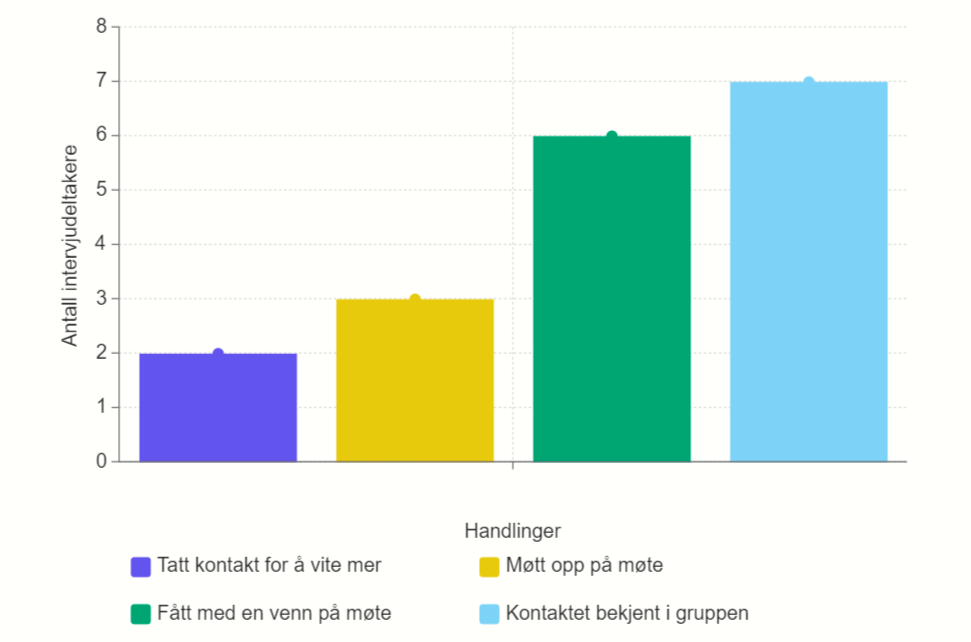
\includegraphics[width=\textwidth]{Illustrasjoner/diagram-handlinger.png}
\caption{Stolpediagram som illustrerer antall intervjudeltakere som ville utført forskjellige handlinger ved funn av interessant aktivitet}
\label{fig:diagram-handlinger}
\end{figure}

Intervjudeltakerne ble presentert et scenario der en aktivitet de er interessert i hadde organiserte møter i nærheten av dem en gang i uka og en bekjent av deltakeren var allerede medlem. Deltakerne ble presentert med forskjellige handlinger og spurt om de ville ha utført handlingene i scenarioet beskrevet ovenfor. Som illustrert i diagrammet i figur~\ref{fig:diagram-handlinger} kom det også her fram at det var viktig for flere av deltakerne å involvere en venn eller bekjent for å kunne delta. Det kom også fram at kun to av åtte deltakere ville tatt kontakt for å vite mer, dermed er det viktig at de har tilgang til utfyllende, relevant og riktig informasjon om aktiviteten uten å trenge å ta kontakt.

\paragraph{Intervju med Anders Midtsundstad}
I intervjuet snakket prosjektgruppen med Anders Midtsundstad om sitt arbeid og hvordan det kunne relatere til prosjektgruppens oppdrag. Metoden Fritid med Bistand ble utviklet av Midtsundstad for å kunne legge til rette for at personer med ulike bistandsbehov kunne få støtte for å kunne delta på fritidsaktiviteter. På metodens nettsted beskrives den slik: \say{Metoden er strukturert gjennom seks trinn for å sikre progresjon inn i en selvvalgt fritidsorganisasjon: 1. Informasjonsmøte, 2. Kartlegging av ønsker og drømmer, 3. Kartlegging av fritidsaktiviteter, 4. Valg av fritidsaktivitet, 5. Finne tilrettelegger, 6. Oppfølgning og evaluering} \footnote{https://www.fritidmedbistand.no/om-metoden.326149.no.html}. 

I intervjuet ble problemstillingen med tilgjengeliggjøring av fritidsaktiviteter for alle tatt opp. Midtsundstad skriver i sin masteroppgave {\em  Tillit, Mestring og Selvoppfatning}: \say{Vårt samfunn endrer seg. Tidligere ble vi født inn i et fellesskap, mens det i dagens samfunn kan være grunn til å snakke om at fellesskap skapes av de som er aktører i et mangfold av slike} \cite{TILLIT:13}. Midtsundstad fortalte om vanskeligheten mange hadde med å være åpen om sine behov for bistand og tilrettelegging, som igjen kunne føre til at de heller unngikk å delta og falt utenfor. Dette kunne gjelde både personer med funksjonsnedsettelser, personer med sosiale vansker og andre. 

Han fortalte at man må etablere et tillitsforhold, slik at når døren til aktiviteten er synlig åpen, så blir det desto lettere å gå igjennom den. Disse dørene kunne bli åpnet av støttekontakter, faddere eller andre frivillige. Etablering av tillitsforhold i tjenesten Aktiv Student ble drøftet med tanke på at det var en digital tjeneste og det kunne vise seg vanskelig å etablere tillit hos brukeren uten menneskelig kontakt og kartlegging av hver enkelt brukers behov.

\paragraph{Intervju med NAV-ansatt}
%Beskrivelse av deltaker: alder, kjønn, bakgrunn%
For å få innspill som kunne være til større hjelp for de mest sårbare personene i målgruppen ble det gjennomført et intervju med en kvinne som jobbet med sosialhjelp i NAV for personer under 30 som ønskes ut i jobb. 

\vspace{5mm} %5mm vertical space

I intervjuet kom det fram at ensomhet var en faktor som man så hos mange av NAV-brukerne. Flere opplevde det som flaut at de ikke hadde flere venner. Det kunne virke som flere trengte {\em  en hånd å holde i} for at de skulle kunne møte opp på arrangementer, det å dra alene syntes mange var skummelt. Det forekom også hos NAV-brukerne at det var vanskelig å initiere kontakt. Det var oftere suksess hvis NAV-kontakten avtalte å ringe NAV-brukeren enn motsatt.


\begin{figure}[H]
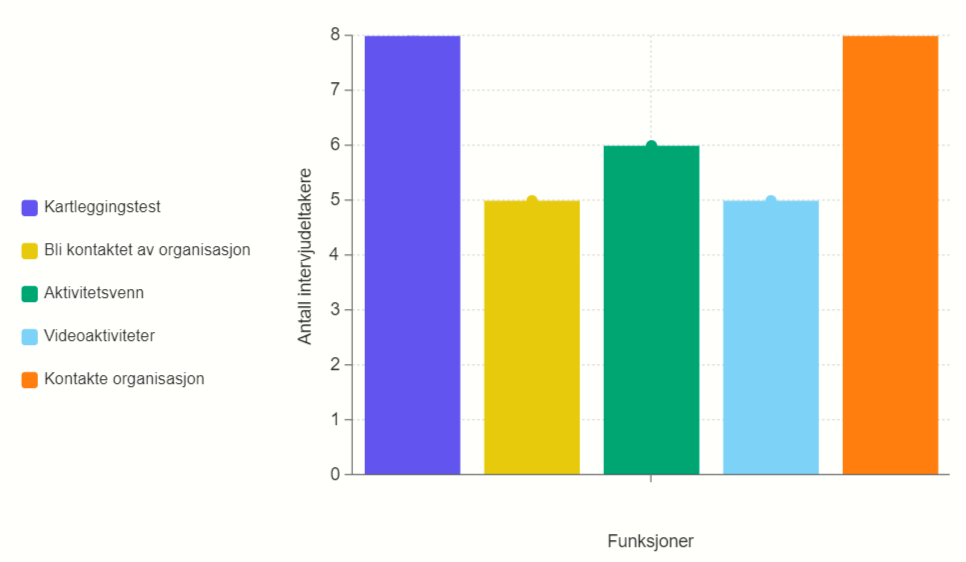
\includegraphics[width=\textwidth]{Illustrasjoner/diagram-funksjoner.png}
\caption{Stolpediagram som illustrerer antall intervjudeltakere som ville brukt funksjoner foreslått av prosjektgruppen.}
\label{fig:diagram-funksjoner}
\end{figure}

\paragraph{Studenter om funksjonalitet i Aktiv Student}

Med utgangspunkt i funksjoner som prosjektgruppen har foreslått ble intervjudeltakerne spurt om de ville brukt disse funksjonene selv. Resultatene er presentert i diagrammet i figur~\ref{fig:diagram-funksjoner}. Kartleggingstesten utmerket seg som en populær idé, én deltaker sa at \say{det gjør nettsiden mer spennende og jeg kan finne noe jeg ikke hadde tenkt på fra før}. Andre deltakere la til at de syntes det var viktig at ikke testen var for lang hvis funksjonen skulle bli brukt.

Å bli kontaktet av en organisasjon, slik prosjektgruppen la fram funksjonen til deltakerne, sto fram som en idé med forbedringspotensiale. Hensikten med funksjonen var å gjøre det enklere for brukere å komme i kontakt med organisasjoner uten å trenge å skrive en e-post eller ringe. Denne hensikten så gruppen på som viktig for tjenestens funksjon. Det kom forslag til forbedring og konkretisering av funksjonen fra en intervjudeltaker. En {\em  ping}-knapp som bruker kunne trykke på for å varsle organisasjonen om at noen var interessert. Dette innspillet tok prosjektgruppen med seg videre.

Seks av åtte intervjudeltakere svarte at aktivitetsvenn-funksjonen var noe de ville ha brukt. Utfordringene med denne funksjonen var at det ikke kunne være flaut eller for høy terskel for brukere å ta kontakt med en potensiell aktivitetsvenn. En tilbakemelding fra en deltaker som ikke ville brukt funksjonen var \say{jeg vil heller ta kontakt med selve organisasjonen enn en ukjent person, men hvis jeg hadde funnet en bekjent hadde jeg brukt funksjonen}. Ettersom det sosiale aspektet og deltakelse sammen med andre var sentralt i prosjektet ble det tydelig at prosjektgruppen måtte jobbe grundig med å finne metoder for å gjøre denne funksjonen så lavterskel og lite truende som mulig. 

Videoaktiviteter svarte fem av åtte intervjudeltakere at de ville brukt. Flere deltakere sa at de helst ville møtes i virkeligheten. Én deltaker svarte at det eneste tilfellet der videoaktiviteter var aktuelt for han var i perioden med restriksjoner på grunn av Covid-19, noe som forhåpentligvis ikke vil bli aktuelt når tjenesten skal utvikles. En annen bruker som sa han ville brukt funksjonen for å \say{blitt med på CV-kurs eller lignende}.

Alle intervjudeltakerne svarte at de kunne selv tatt kontakt med en organisasjon så lenge organisasjonens kontaktinformasjon var lett tilgjengelig.

\begin{figure}[H]
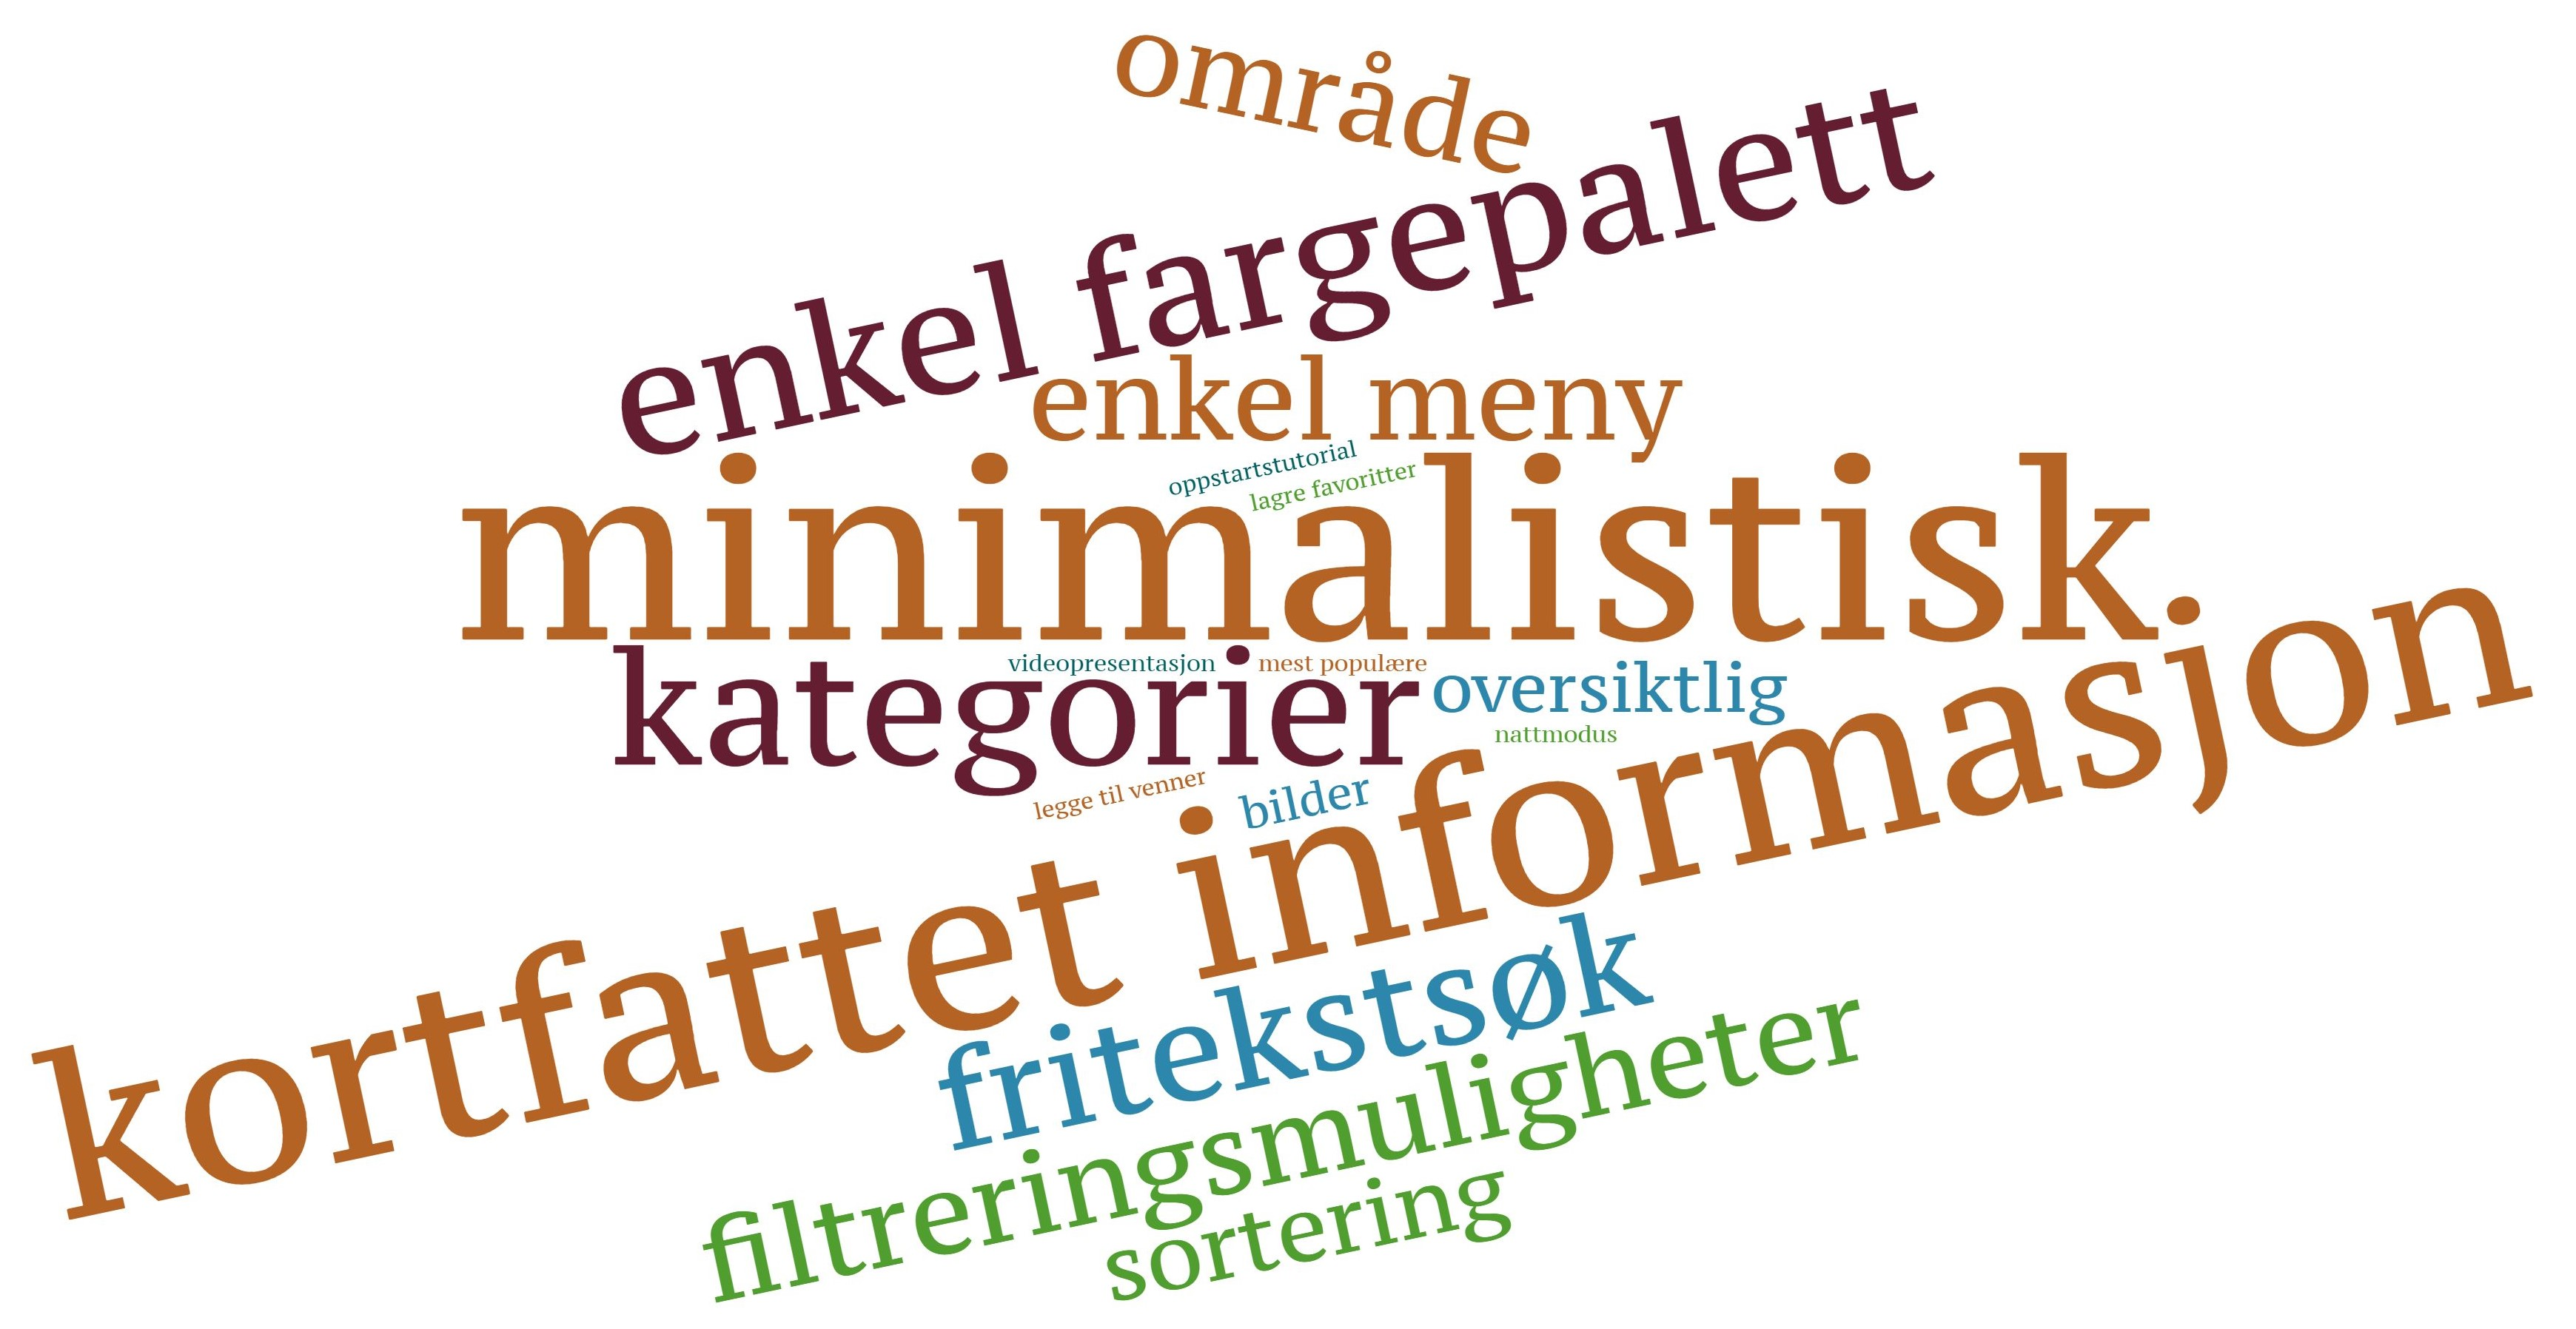
\includegraphics[width=\textwidth]{Illustrasjoner/ordsky-funksjoner.jpg}
\caption{Ordsky som viser hva som var viktig for dem i den tekniske implementasjonen av tjenesten.}
\label{fig:ordsky-funksjoner}
\end{figure}

Avslutningsvis ble intervjudeltakerne spurt om hvilke funksjoner, designvalg og tekniske løsninger de syns var viktig for at tjenesten skulle bli god, de oftest nevnte svarene er illustrert i en ordsky i figur~\ref{fig:ordsky-funksjoner}. 

Fritekstsøk, kategorisøk og filtrering var noen av de konkrete funksjonene som gikk igjen hos intervjudeltakernes svar. Disse funksjonene ser også prosjektgruppen på som de mest grunnleggende funksjonene i tjenesten. Flere deltakere nevnte at de ville ha mulighet til å filtrere på hvilket område aktiviteten foregikk. Funksjoner som videopresentasjon av organisasjoner og oversikt over mest populære aktiviteter ble også foreslått av deltakere.

Alle deltakere kom fram til at de ønsket et minimalistisk og oversiktlig design med kun den nødvendige informasjonen. Én deltaker sa at han ønsket \say{en egen side der folk kan lese utfyllende info hvis de trenger det, i stedet for en blokk med tekst som nesten ingen leser}. En annen ville ha \say{all viktig info man trenger på en full side uten å måtte scrolle}. Alle deltakere mente at mange farger var forstyrrende. Fargepaletten burde være enkel, men ikke kjedelig. Flere svarte at menyen burde være så enkel som mulig med konkrete, tydelige valg og få eller ingen undermenyer.

\subsection{Oppfølgingsintervju om spesifikke funksjoner}
Etter gjennomføring av intervjuer satte prosjektgruppen i gang med å utarbeide forslag om hvilke funksjoner som skulle være med i tjenesten. På noen punkter var prosjektgruppen uenig om funksjonene skulle være med eller ikke. På andre punkter trengte gruppen flere ideér om hvordan en funksjon kunne forbedres og revideres. På disse punktene var det heller ingen klare svar fra brukerintervjuer som pekte mot hva brukeren ønsket. Det ble derfor gjennomført et kort oppfølgingsintervju med fem studenter, hvorav to av disse ikke hadde deltatt i de initielle brukerintervjuene. Prosjektgruppen ønsket å finne ut om deltakerne mente at funksjonene

\begin{enumerate}
\item Var viktig for tjenestens hensikt
\item Ville bli brukt
\item Ikke brøt med det minimalistiske konseptet
\end{enumerate}

Deltakerne ble konsultert på tre funksjoner: kontakt mellom bruker og organisasjon, mest populære aktiviteter og filtrering på hvilke dager de forskjellige gruppene har møter.

\paragraph{Hvordan enklest initiere kontakt mellom bruker og organisasjon?} 
På grunnlag av relevante studier % legg inn kildehenvisninger her %
, konsultasjon med fagperson Anders Midtsundstad \cite{MIDTSUNDSTAD-INTERVJU:15} og intervju av en NAV-ansatt \cite{NAV-INTERVJU:16} ble det konkludert med at det var viktig å ha en lavterskel løsning som gjorde det lite truende å initiere kontakt mellom brukere og organisasjoner.

Den første løsningen, en {\em  kontakt meg}-knapp på organisasjonens side, var ikke godt nok gjennomtenkt og medførte flere begrensninger. Det var for eksempel ikke tenkt på hvordan organisasjonen skulle bli varslet om at de skulle kontakte noen, spesielt om de ikke hadde ressurser til å sjekke varsler så ofte. Det satte for mye av ansvaret over på organisasjonene. Hvis en person ikke hadde blitt kontaktet, skulle organisasjonen da holdes ansvarlig?

De fem deltakerne av oppfølgingsintervjuet ble spurt om ideér til hvordan man kunne gjennomføre en slik lavterkel løsning uten disse begrensningene. De fleste av deltakerne kom fram til at den mest effektive måten å initiere kontakt på var at organisasjonen fikk e-post. Det ble også nevnt at det var viktig å informere brukeren om at ikke alle organisasjoner har like store ressurser, så det var ikke sikkert at de fikk svar med en gang om de valgte å ikke ta direkte kontakt. Det ble lagt vekt på at ansvaret med en slik funksjon ikke skulle ligge hos organisasjonen, men skulle være et supplerende tilbud for kontakt for brukeren. 

Den mest hensiktsmessige løsningen ble foreslått av en intervjudeltaker og utviklet videre av prosjektgruppen. Denne løsningen var en {\em ping} funksjon. Brukeren kunne {\em pinge} en organisasjon, informert om at det var ingen garanti om at organisasjonen svarte på kontakten. Organisasjonen får da tilsendt en standardisert e-post om at en bruker er interessert i organisasjonen deres og gjerne vil vite mer, inkludert brukerens e-post adresse. For organisasjonen vil det være like enkelt å svare på en slik e-post som å svare på en e-post sendt direkte fra en bruker. For brukeren kan det virke mye mindre skremmende og kreve mindre innsats å trykke på {\em ping}-knappen enn å formulere en e-post for å initiere kontakt.

\paragraph{Mest populære aktiviteter-funksjonen}
Dette var en funksjon som ble foreslått av en deltaker under de initielle brukerintervjuene. Forslaget gikk ut på å vise en oversikt over de tre til fire mest populære aktivitetene på tjenesten, enten på forsiden eller når man velger en spesifikk kategori. Hensikten med dette var at brukeren skulle ha et sted å starte på tjenesten, hvis den ikke visste spesifikt hva den lette etter. Et annet poeng var at det kunne være større sjanse for at brukere tør å møte opp på aktiviteter hvis de visste at det var mange andre som skulle komme.

\begin{figure}[H]
\fbox{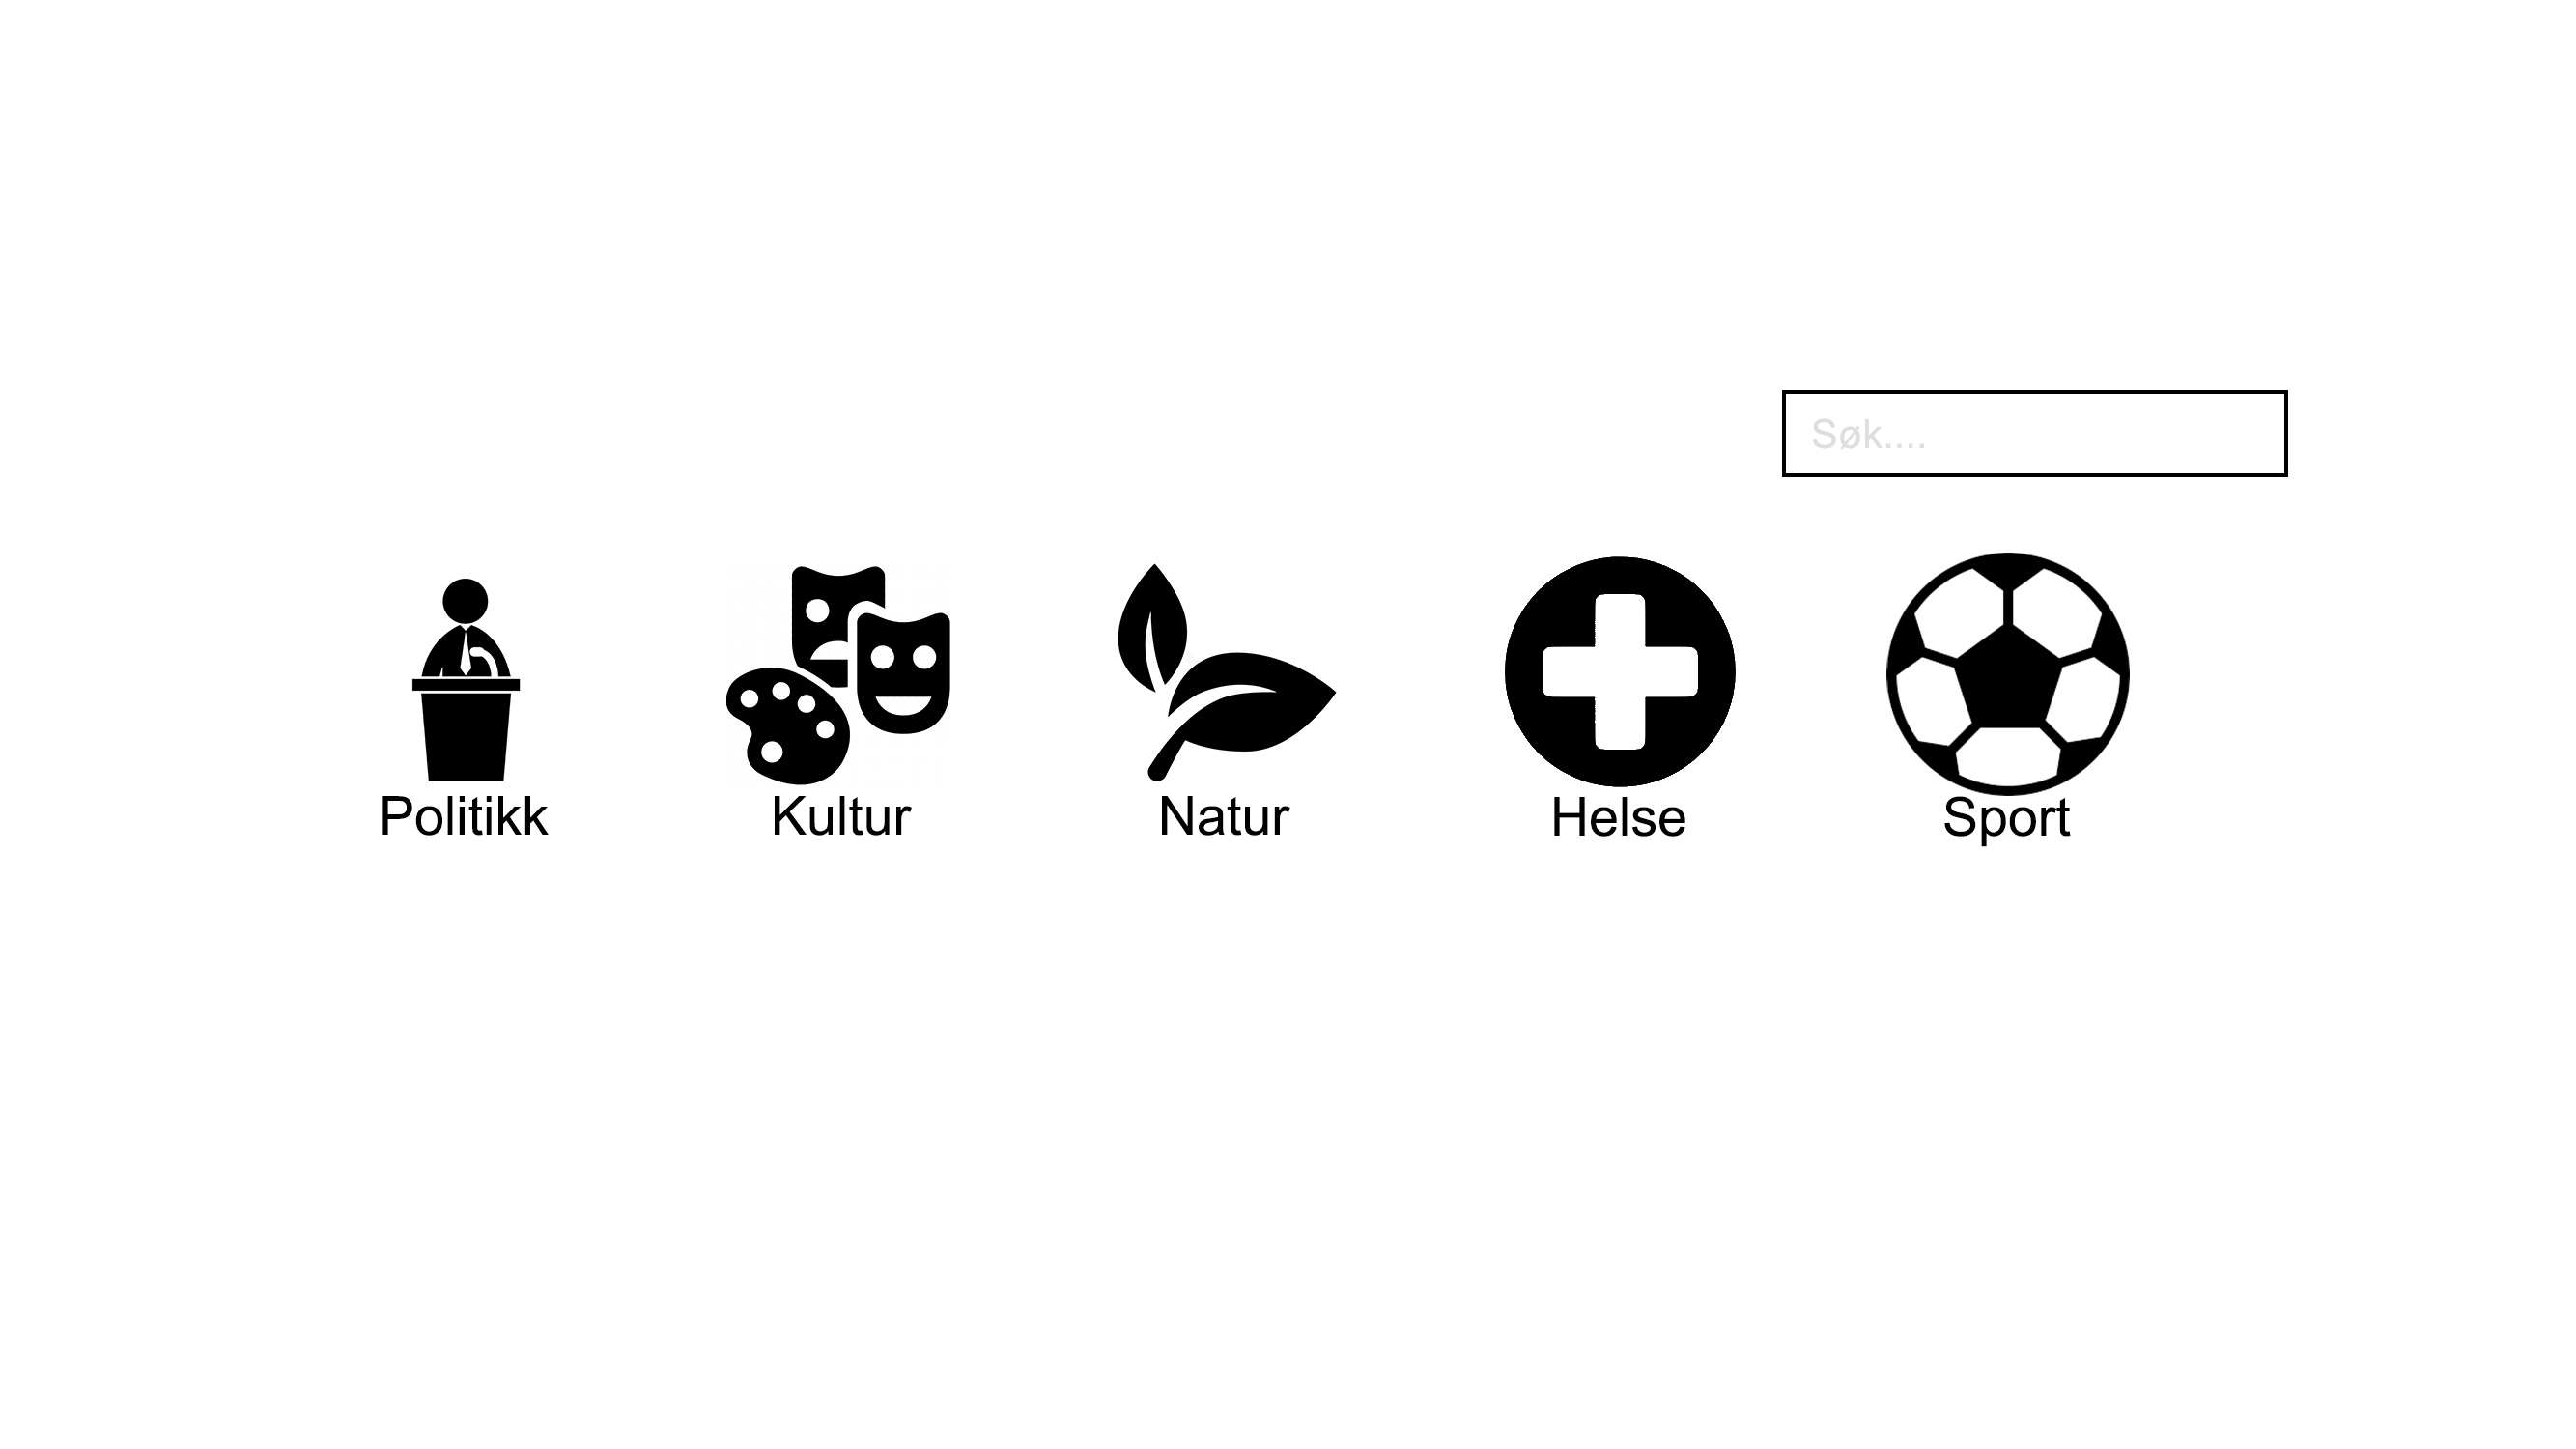
\includegraphics[width=\textwidth]{Illustrasjoner/sketch-uten-aktiviteter.jpg}}
\caption{Skisse av forside uten visning av mest populære aktiviteter}
\label{fig:utenMestPopulaere}
\end{figure}

\begin{figure}[H]
\fbox{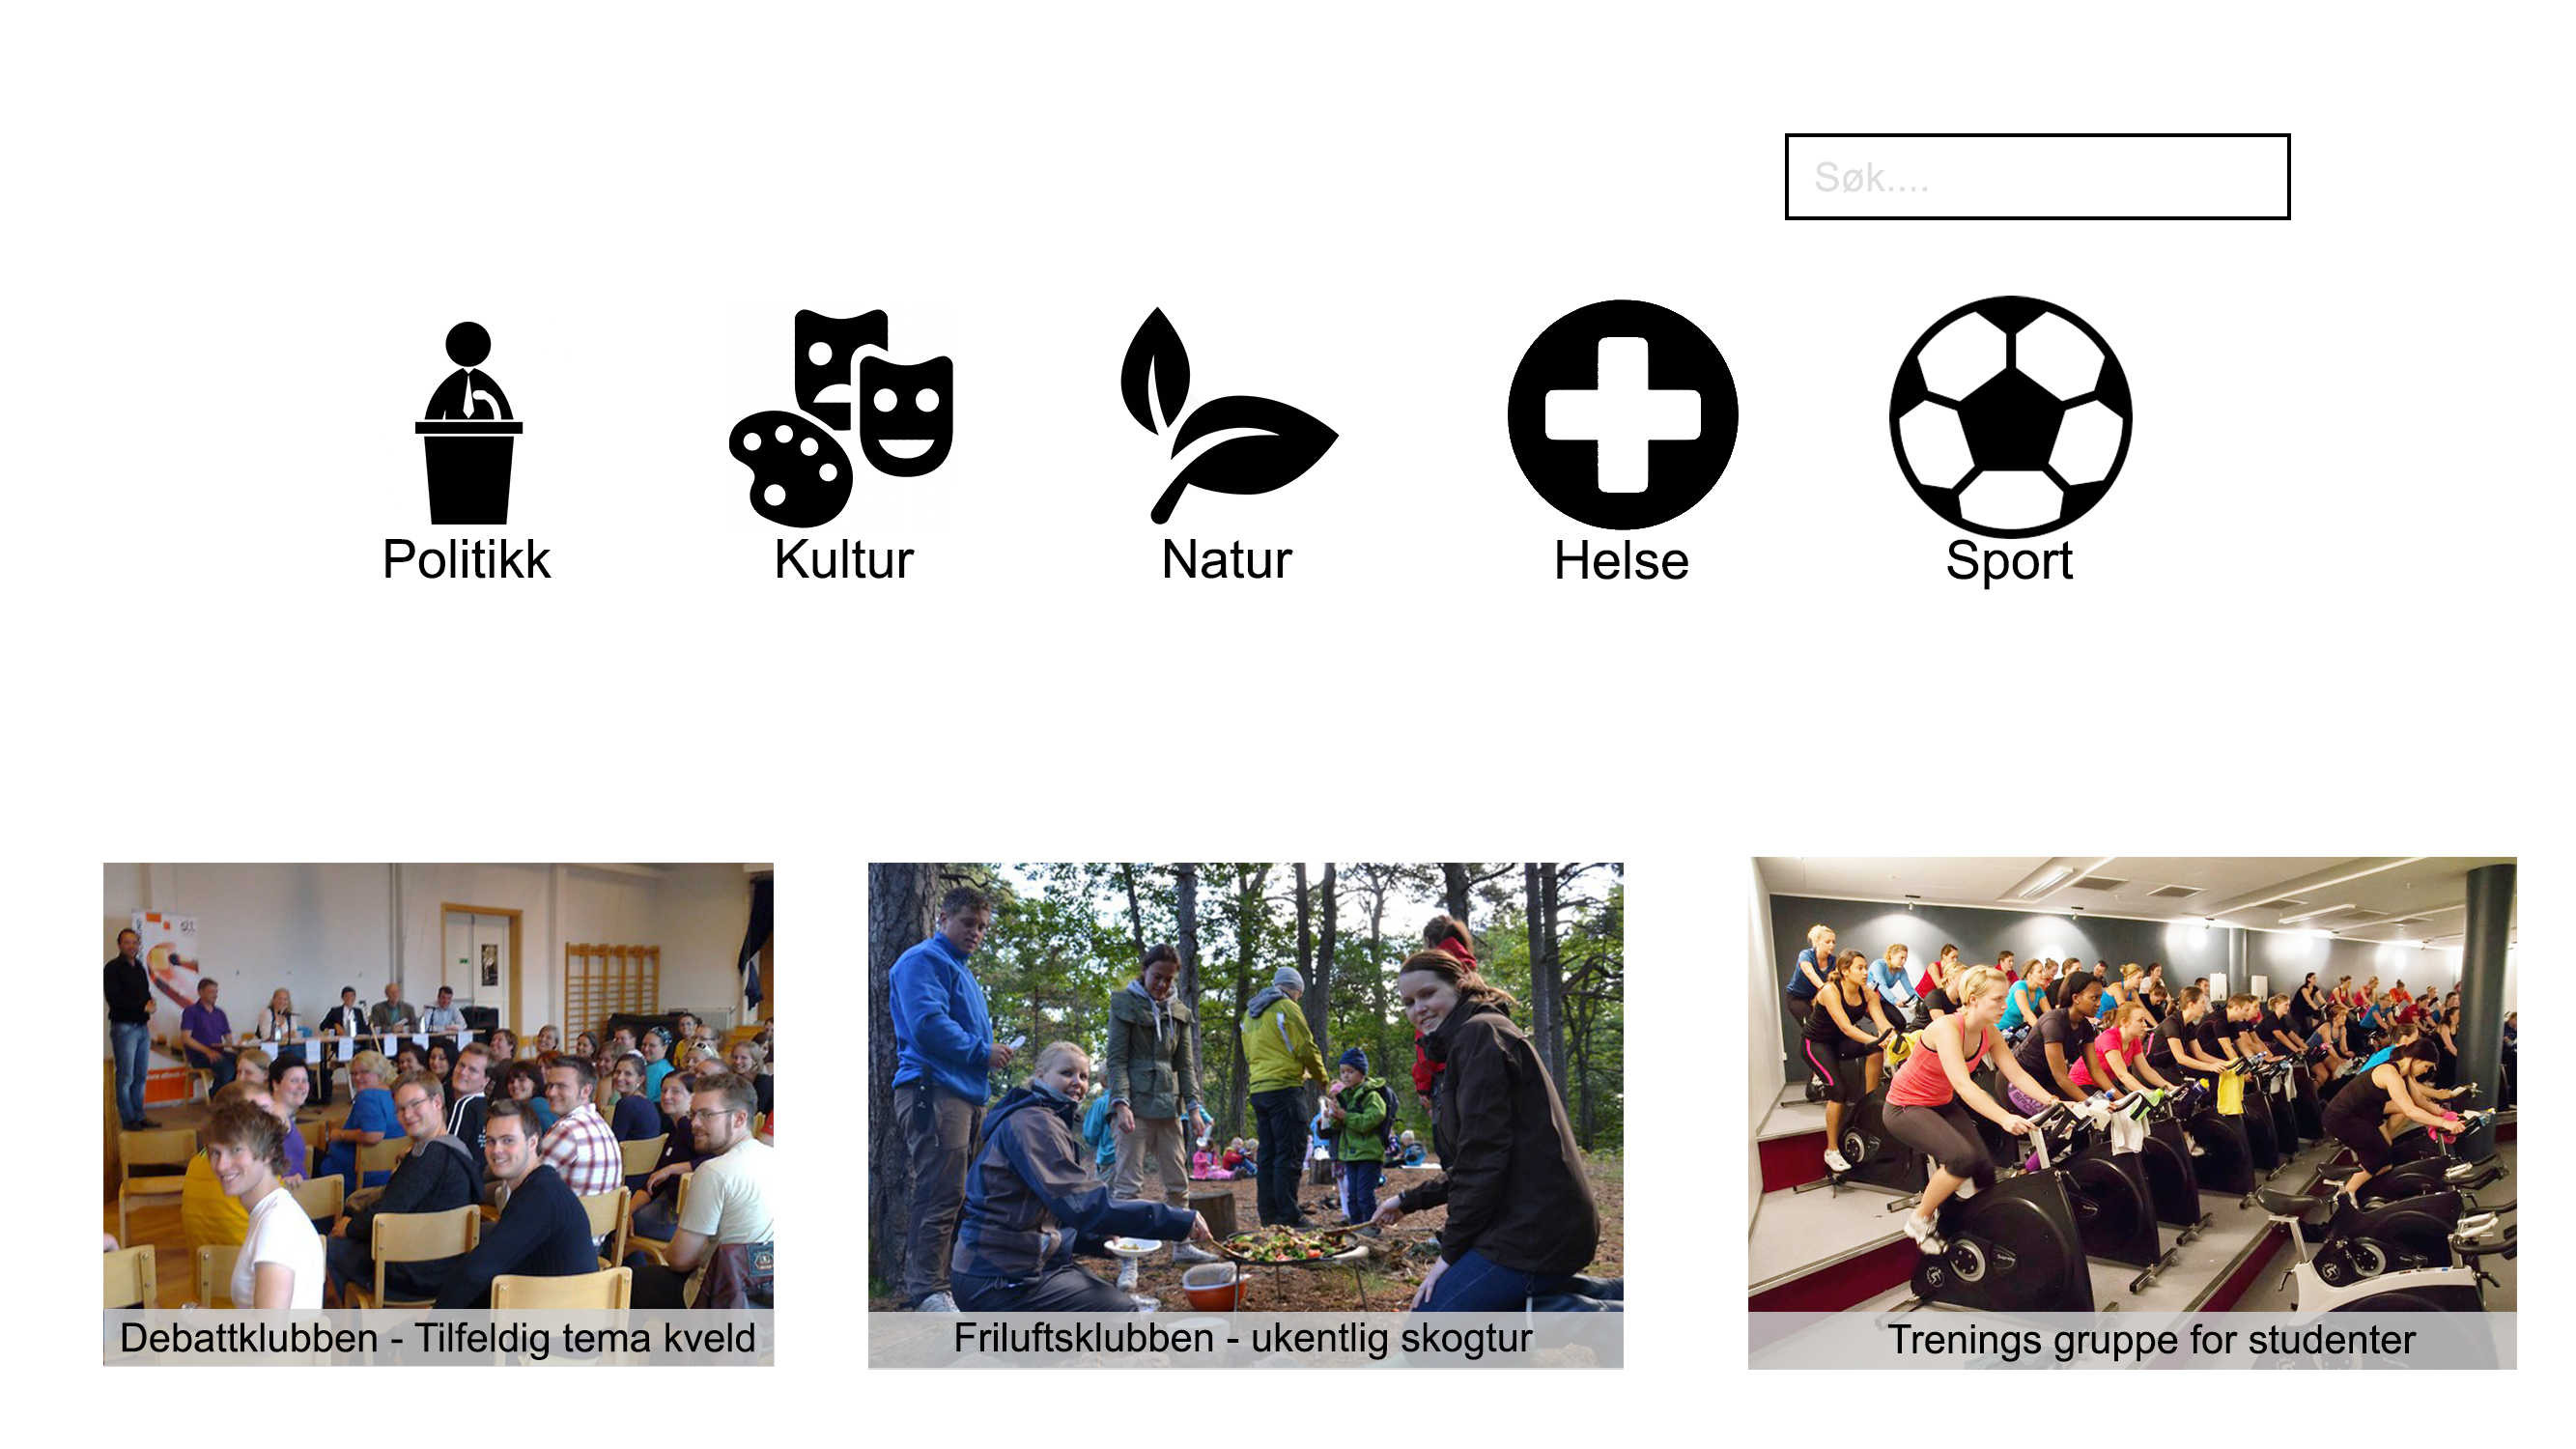
\includegraphics[width=\textwidth]{Illustrasjoner/sketch-med-aktiviteter.jpg}}
\caption{Skisse av forside med visning av mest populære aktiviteter}
\label{fig:medMestPopulaere}
\end{figure}

Det ble laget enkle skisser av en forside med og uten visning av mest populære aktiviteter. Figur~\ref{fig:utenMestPopulaere} illustrerer hvordan forsiden kunne sett ut uten mest populære aktiviteter og figur~\ref{fig:medMestPopulaere} illustrerer hvordan den kunne sett ut med denne funksjonen. Skissene skulle hjelpe deltakerne av oppfølgningsintervjuet å komme fram til om de syntes at funksjonen virket forstyrrende for layout og om det brøt med minimalisme-konseptet.

Tilbakemeldingene fra deltakerne var blandede. Noen mente at funksjonen ikke var sentral for tjenestens hensikt, andre mente at den kunne gjøre terskelen lavere for å bli med og at å presentere brukeren med en aktivitet med én gang kan øke muligheten for at brukeren blir på tjenesten. Skissen med visning av mest populære aktiviteter, vist i figur~\ref{fig:medMestPopulaere}, ble ikke sett på som forstyrrende og brøt ifølge deltakerne ikke med det minimalistiske konseptet. 

Ettersom tilbakemeldingene var blandede bestemte prosjektgruppen seg for å lage mer detaljerte skisser av funksjonen og brukerteste dem videre i neste runde med brukerundersøkelser før det ble bestemt om funksjonen skulle være med eller ikke.

\paragraph{Filtrering på møtedager}
I de initielle brukerintervjuene hadde flere svart at de ønsket å kunne se hvilke dager og tider organisasjonene hadde møter. For å kunne videre fasilitere for dette ble det av prosjektgruppen foreslått en mulighet for å filtrere på hvilke dager organisasjonene har møter om brukeren velger å søke med filtrering. Dette ville da komme i tillegg til at brukeren kunne se møtetidene på organisasjonens profil. 

Dette ble foreslått for å kunne gjøre det enklere for brukere med begrensede muligheter til å møte opp, for eksempel brukere med barn eller jobb. Om disse brukerne kun kan møte opp én eller to dager i uka var ideén at de skulle slippe å gå inn på hver organisasjons profil for å sjekke møtetider, men heller filtrere vekk de uaktuelle organisasjonene med én gang.

En ulempe som med funksjonen som ble tatt opp var at i startfasen til tjenesten hadde kanskje ikke så mange av organisasjonene lagt inn møtetidspunkter. Hvis en bruker valgte å filtrere på møtetider, skulle kun de få som har lagt inn tider og matcher med søket vises, eller skulle også de som enda ikke hadde lagt inn tider dukke opp i resultatene?

Ikke alle av deltakerne på oppfølgingsintervjuet hadde behov for å bruke funksjonen selv, men alle kunne se for seg at dette kunne være en viktig funksjon for brukere som hadde mindre fleksibilitet når det kom til fritid. Deltakerne var enige i at funksjonen kunne bidra til å senke terskelen og inkludere disse brukerene i aktiviteter. Derfor bestemte gruppen seg for å beholde denne funksjonen.

\section{Første forslag til tjenestens funksjoner og innhold}

Før arbeidet med å prototype fysiske skisser ble satt i gang måtte det lages en liste over alt som skulle være med i tjenesten. Listen inneholdt i utgangspunktet alle ideér til funksjonalitet fra brukere i brukerintervjuer, medlemmer av prosjektgruppen, ideér fra relevant forskning og studier og reviderte funksjoner som ble endret på etter brukerintervjuer. Deltakerne av brukerintervjuene la vekt på at de ønsket en minimalistisk tjeneste med kun det mest nødvendige innholdet, dette var et viktig fokusområde for prosjektgruppen under utviklingen av første forslag til tjenesten.

\subsection{Brukerens kravspesifikasjon}
\label{section:kravspec}
Etter å ha gjennomført de initielle intervjuene ble det laget en kravspesifikasjon som oppsummerte hva som var viktig for brukeren å ha med i tjenesten av innhold og funksjonalitet.

\paragraph{Tjenestens innhold}
\begin{compactitem}
\item Det skal være enkelt å finne oversikt over tilgjengelige aktiviteter
\item Det skal være enkelt å søke på og finne fram til en spesifikk aktivitet
\item Systemet skal hjelpe brukeren å finne potensielle aktiviteter som passer for den
\item Informasjonen skal være oppdatert og korrekt
\item Det skal være relevant og utfyllende informasjon om aktivitetene
\item Det skal være enkelt å komme i kontakt med organisasjoner
\item Det skal være lav terskel for å komme i kontakt med organisasjoner
\item Det skal være enkelt å ta kontakt med andre brukere
\item Det skal være lav terskel for å ta kontakt med andre brukere
\item Systemet skal fasilitere for at brukere kan delta på aktiviteter sammen
\item Systemet skal være spennende og attraktivt å bruke
\end{compactitem}

\paragraph{Teknisk funksjonalitet}
\begin{compactitem}
\item Det skal gå an å filtrere søk på relevante kriterier
\item Tjenesten skal være intuitiv og gjenkjennelig
\item Designet skal være minimalistisk
\item Det skal være enkelt å finne fram dit man skal i tjenesten
\item Innholdet som vises skal være kun det nødvendige
\item Tjenesten skal ikke inneholde forstyrrende funksjoner eller designmomenter
\item Fargepaletten skal være enkel og minimal
\item Menyen skal kun inneholde det nødvendige
\item Søkefeltet skal være synlig og lett tilgjengelig
\end{compactitem}

\subsection{Liste over funksjoner}
\label{section:forslag1-liste-over-funksjoner}
I arbeidet med å velge hvilke funksjoner som skulle være med i første forslag til tjenesten var hensikten å kun jobbe videre med idéene som var nødvendige, bygget opp under tjenestens egentlige hensikt og direkte jobbet opp mot å løse problemstillingen.

Enkelte av idéene ble strøket fra listen med en gang, ikke fordi de var dårlige, men fordi det var tydelig at det ikke var sentrale for tjenestens hensikt. Eksempler på slike funksjoner var:

\begin{itemize}
    \item Legge til venner man kjenner fra før
    \item Oppstartsanvisning til nye brukere
    \item Legge til aktiviteter i en {\em favoritter}-mappe
\end{itemize}

Andre ideer ble strøket av listen eller endret på fordi svarene fra brukerintervjuene pekte mot at de i stor grad ikke ville bli brukt. Noen av disse var:

\begin{itemize}
    \item Videoaktiviteter
    \item Organisasjon tar kontakt med bruker
\end{itemize}

Etter å ha eliminert unødvendige funksjoner sto prosjektgruppen igjen med denne listen over funksjoner som skulle være med i videre arbeid av tjenesten:

\begin{center}
\begin{longtabu}{|X|X|}
\caption{Liste over funksjoner og hensikten med disse} \label{tab:funksjoner} \\

\hline \multicolumn{1}{|c|}{\textbf{Funksjon}} & \multicolumn{1}{c|}{\textbf{Hensikt}} \\ \hline 
\endfirsthead

\multicolumn{2}{c}%
{{\bfseries \tablename\ \thetable{} -- fortsettelse}} \\
\hline \multicolumn{1}{|c|}{\textbf{Funksjon}} & \multicolumn{1}{c|}{\textbf{Hensikt}} \\ \hline 
\endhead

\endlastfoot

Innhenting av informasjon om organisasjoner fra Brønnøysundregistrene 
& tjenestens datakilde \\ \hline

Oppfordring av organisasjoner til å opprette profil og legge inn mer info 
& Gir brukeren utfyllende og nyttig informasjon om organisasjonen \\ \hline

Brukere kan opprette brukerprofil 
& Gir bruker mulighet til å legge inn informasjon om seg selv og kontakte en aktivitetsvenn \\ \hline

Kartleggingstest med
\begin{compactitem}
    \item Oversikt over relevante organisasjoner
    \item Mulighet for kontakt med organisasjoner
    \item Mulighet for å se mer info om organisasjoner
    \item Mulighet til å finne aktivitetsvenn med samme interesse
\end{compactitem}
& Gjøre det enkelt og spennende for brukeren å oppdage nye organisasjoner og aktivitetsvenner \\ \hline

Legge til aktivitetsvenner & 
Gjøre det mindre skremmende og mer motiverende for bruker å møte opp på aktiviteter gjennom å delta sammen med noen andre \\ \hline

Bruker kan enkelt ta kontakt med organisasjoner
\begin{compactitem}
    \item Ping-funksjon
    \item Tilgjengelig kontaktinfo
    \item Oppfordre organisasjon til å legge til flere måter å ta kontakt på og være tilgjengelig
\end{compactitem}
& Øke sjansen for at en bruker kontakter en organisasjon og deltar på aktiviteter \\ \hline

God informasjon om aktiviteter 
\begin{compactitem}
    \item Kalender med møtetider
    \item Videopresentasjon eller bildegalleri
    \item Har medlemskontigent/har ikke medlemskontigent
    \item Inkluderende ordbruk
    \item Oversiktlig
    \item Plassering og kart
\end{compactitem}
&  Gi brukeren nok informasjon til at den føler seg trygg på å ta kontakt med organisasjonen og/eller delta\\ \hline

Fritekstsøk
& Gi brukeren mulighet til å utføre et målrettet søk på spesifikke aktiviteter \\ \hline

Filtrering på
\begin{compactitem}
    \item Område
    \item Kategori
    \item Møtedager
\end{compactitem}
& Gi brukeren mulighet til å utføre et målrettet søk etter kriterier som kan være viktig for den \\ \hline

Velge kategori og se aktiviteter
& Brukere som vet hvilke type aktiviteter de er interessert i kan oppdage hvilke tilbud som fins innen disse kategoriene \\ \hline

Mest populære aktiviteter (må brukertestes videre) 
& Presentere brukere med et tilbud uten at de trenger å gjøre noe, gi brukeren et tilbud der de vet det er mange deltakere \\ \hline

\end{longtabu}
\end{center}

\subsection{Sitemap}

\begin{figure}[H]
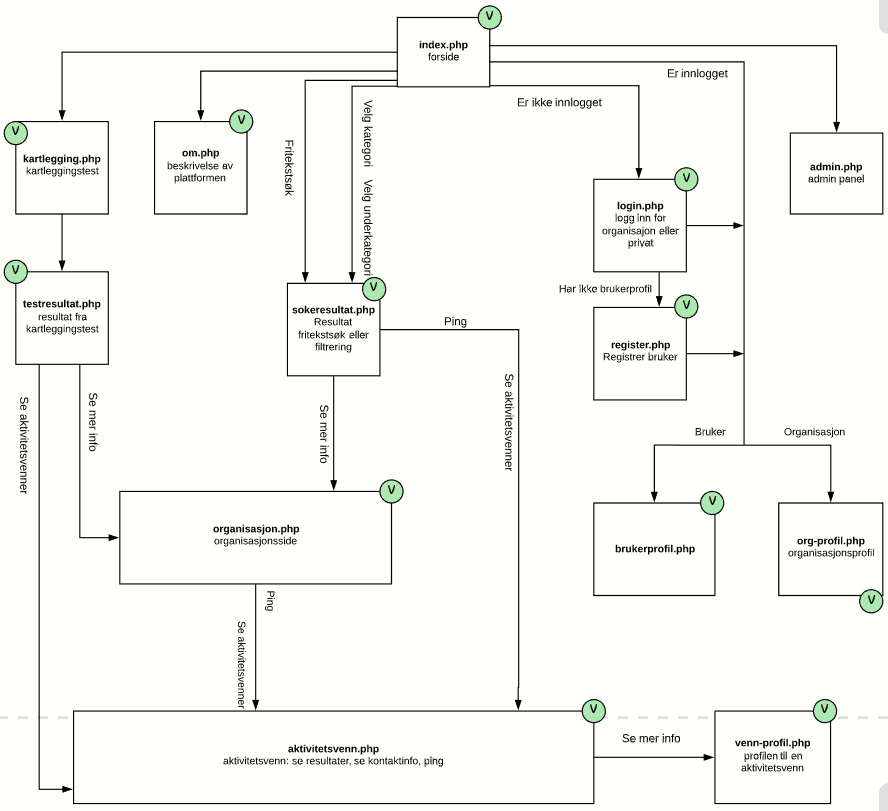
\includegraphics[width=\textwidth]{Illustrasjoner/trehierarki.png}
\caption{Diagram som viser tjenestens sidehierarki}
\label{fig:trehierarki}
\end{figure}

% skrive litt om hvordan vi kom fram til sidehierarkiet og hva det viser %


\subsection{Utforming av skisser versjon 1.0}
\label{section:utforming-1}


Det ble tegnet enkle skisser av alle sidene beskrevet i sidehierarkiet for å få et visuelt inntrykk av tjenesten og dens arkitektur.

Et av punktene som kom fram av brukerintervjuene var ønsket om å kunne delta på en aktivitet uten å trenge å kontakte organisasjonen først. Gjennom å designe funksjonalitet som oppfordret organisasjoner til å legge til informasjon som en student trengte for å kunne møte direkte opp på aktiviteten ville det legge til rette for at studenter som ikke ønsket å ta kontakt av denne årsaken kunne slippe det.

For å kunne skape en tjeneste som var noe mer enn oppslagsverket i Frivillighetsregisteret ble funksjoner utviklet med den hensikt å gjøre tjenesten interessant og spennende, samtidig som funksjonene skulle underbygge tjenestens formål. I prosjektgruppens første forslag til utforming og skisser versjon 1.0 ble kartleggingstesten og aktivitetsvenn-konseptet utformet for å fungere som de spennende funksjonene. Det ble laget to forslag til utforming av kartleggingstesten, dette var fordi prosjektgruppen ikke var sikker på om første versjon av testen fungerte til sin hensikt.

I gjennomføringen av første brukerundersøkelse gjennom Google Forms, beskrevet i delkapittel~\ref{section:google-forms-test} kom det fram at lokasjonen til en aktivitet var informasjon som var viktig for deltakerne. 60\% av deltakerne svarte at de ønsket å kunne snevre inn søket til resultater som var nære området de befant seg i og 80\% ville ønsket å se oversikt over transporttilbud om de var nye tilflyttende studenter. For å fasilitere for dette ble det skissert en løsning der organisasjoner kunne integrere kart fra Google Maps \footnote{https://www.google.com/maps/} på sidene sine. Ved bruk av Google Maps kunne brukerne enkelt få mulighet til å se hvor langt unna de var fra aktiviteten og transporttilbud for å komme seg dit. Det ble også lagt til mulighet for å snevre inn søket til aktiviteter i nærheten av brukeren med en {\em  nær meg}-sjekkboks i filtreringen.

Når resultatene av brukerundersøkelsen ble satt sammen med kravspesifikasjonen kom gruppen fram til de første designvalgene for utformingen av de første skissene.
Det måtte være et simpelt design fylt med ting som var viktig å ha med, ikke ha med masse fine greier som bare ser fint uten å være nødvendig for at siden skal fungere. Det måtte også gjøres plass til ting som brukerene synes var viktig eller kunne fungere, som f.eks {\em Nær meg} funksjonen og gjøre plass til Google Maps.
% skrive mer om utformingen av skissene %

\section{Moderert brukertest av skisser versjon 1.0}
\label{section:Moderert brukertest-skisser-1}

Brukertesten ble gjennomført med fire deltakere som vurderte skissene sammen i gruppe. Hensikten med testen var å finne ut hva deltakernes førsteinntrykk av tjenestens innhold, layout og arkitektur er basert på de enkle skissene. Samt generell oppfatning av konseptet og om det skisserte innholdet bygger opp under prosjektets hensikt. Deltakerne ble bedt om å samarbeide, interagere, spørre og diskutere. Selv om de arbeidet i gruppe ble de bedt om å gi sin personlige mening og ikke {\em henge seg på} en annen deltakers mening. For å få en reell oppfatning av deltakernes førsteinntrykk ble de oppfordret til å si akkurat hva de tenkte og spørre om alt de lurte på uten å bekymre seg for om det hørtes dumt ut.

%Beskrivelse av deltakere: alder, kjønn, bakgrunn%

\begin{figure}[H]
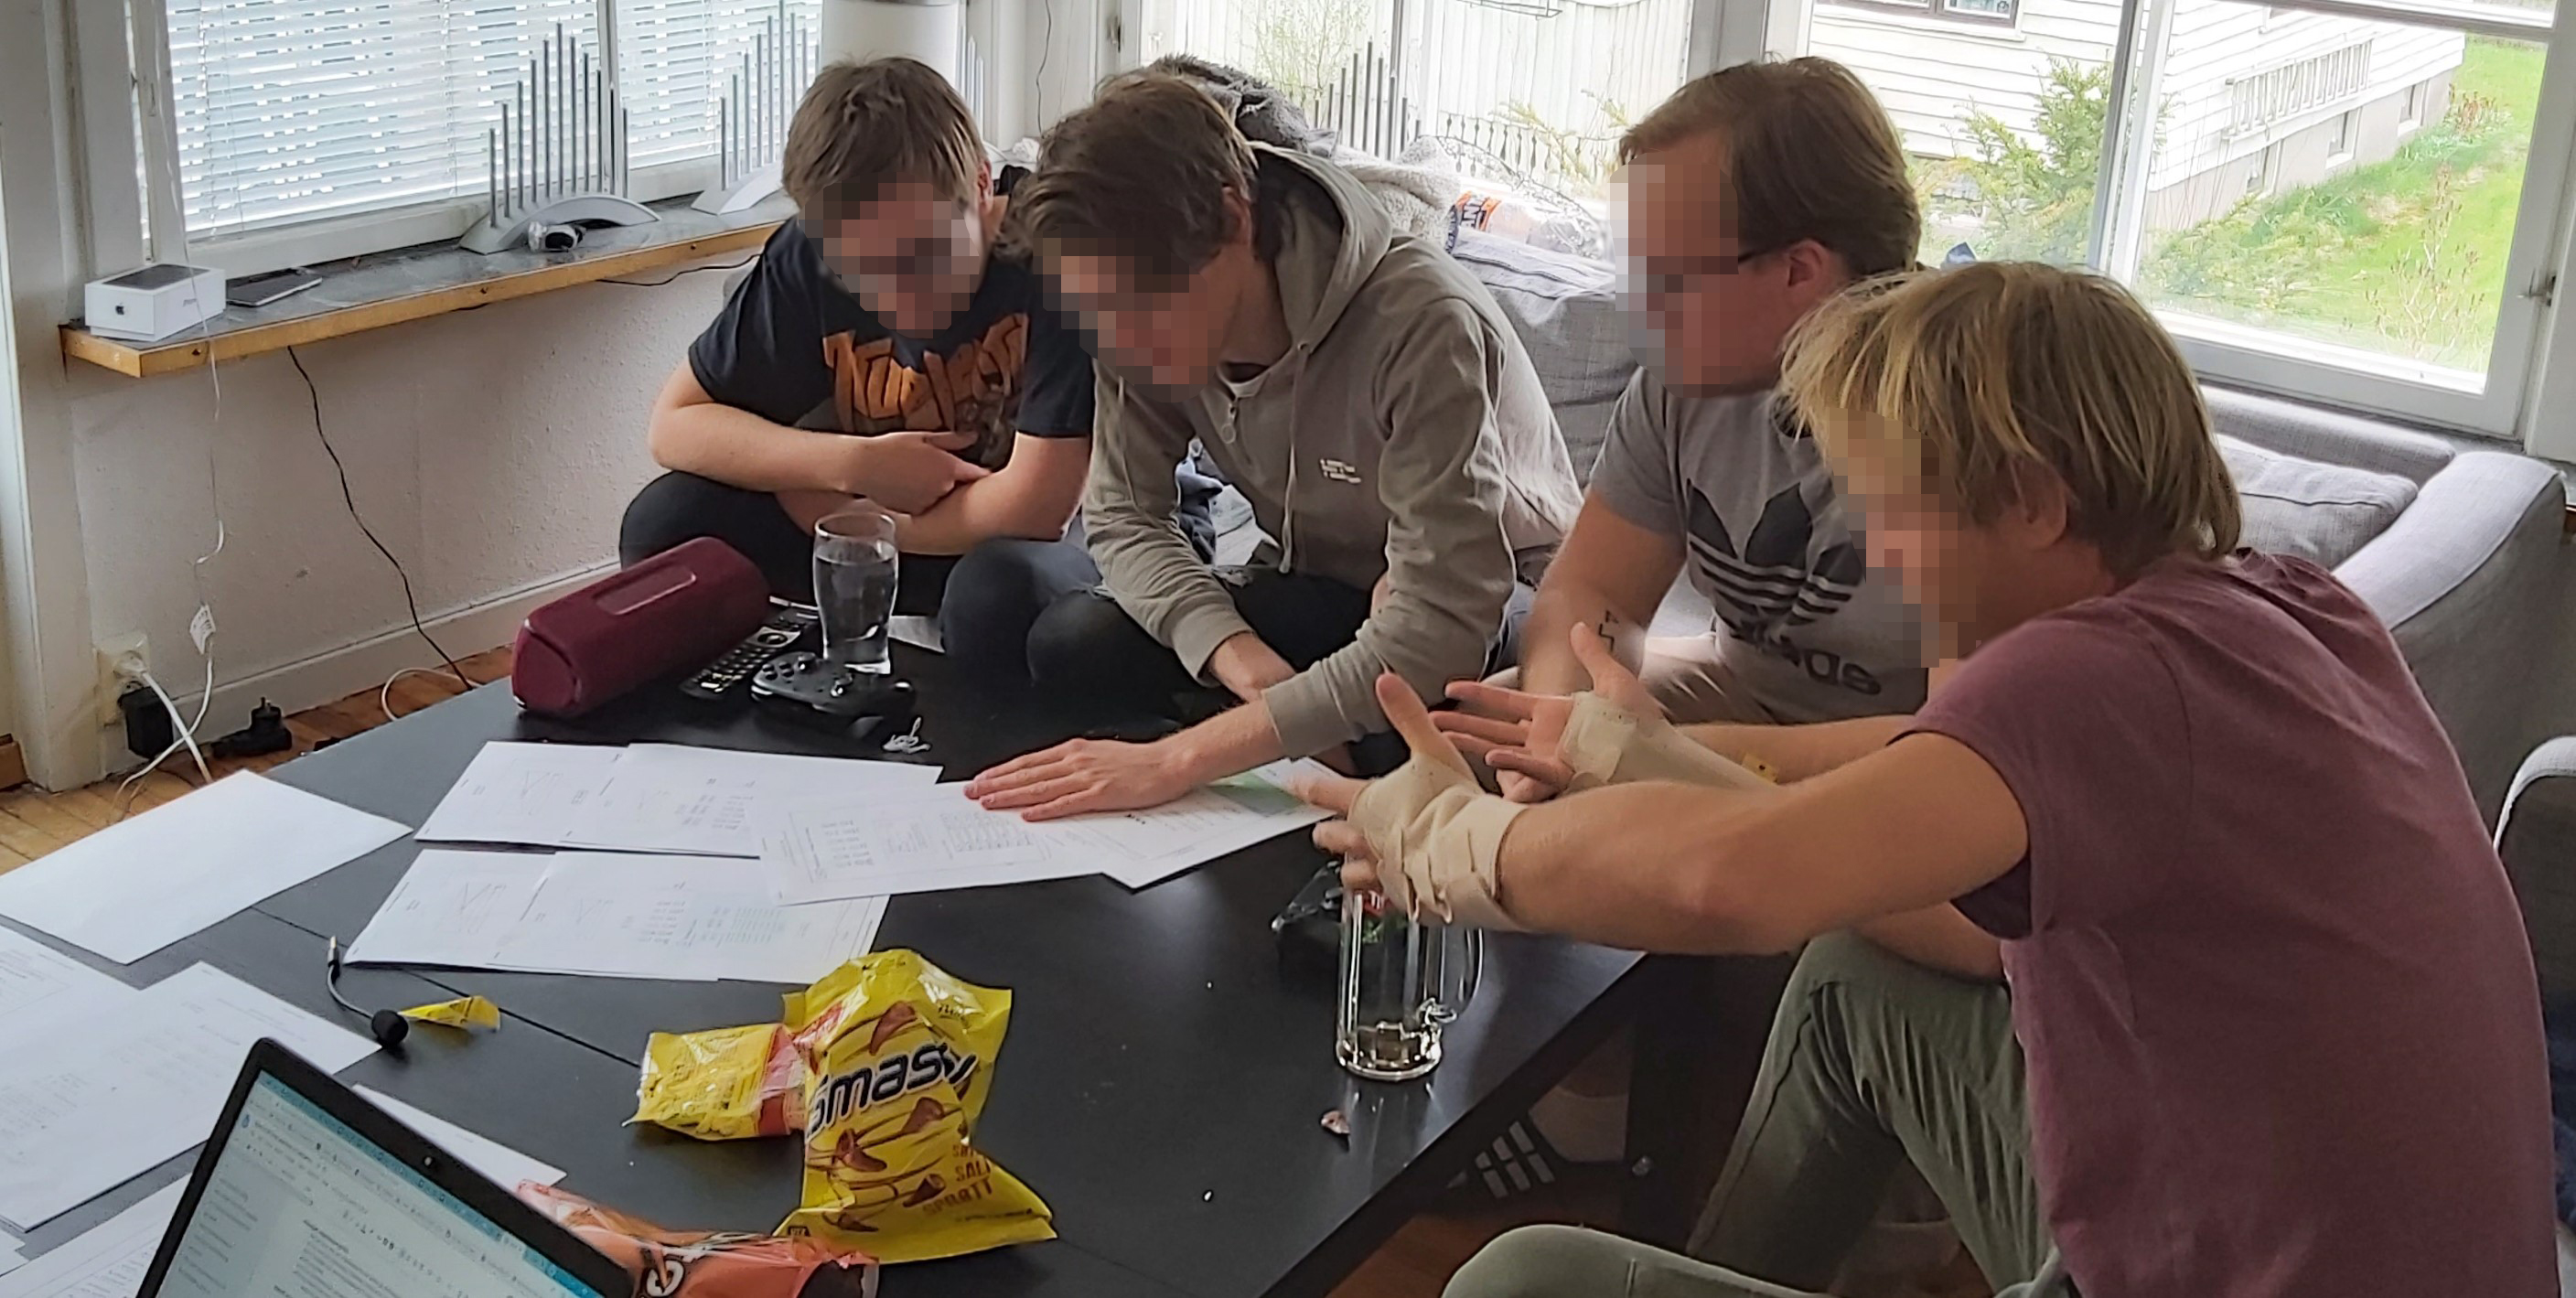
\includegraphics[width=0.8\textwidth]{Illustrasjoner/skissetest-bilde.jpg}
\centering
\caption{Deltakerne av førsteintrykkstesten i prosessen med å diskutere skissene}
\label{fig:skissetest}
\end{figure}

Én og én skisse ble lagt fram i papirformat på bordet foran deltakerne, som vist på bildet i figur~\ref{fig:skissetest}. Da deltakerne ble vist en ny skisse ble de bedt om å si hva deres førsteinntrykk var av hva slags side det var og hva den kunne brukes til. De ble deretter spurt om det var noe de syntes manglet eller om det var noe innhold som var unødvendig, samt om det var noe de ville ha endret på. Brukerne fikk lov å simulere handlinger ved å spørre hva som skjedde hvis man trykket på knapper eller navigerte til andre sider. Da ble de bedt om å si hva de trodde kom til å skje før de ble forklart hva som faktisk ville skje og vist skissen de da hadde navigert til.

For skisser som illustrerte to forskjellige versjoner av samme side eller funksjon ble brukerne bedt om å sammenligne de to versjonene og peke på styrker og svakheter ved de ulike skissene. Etter dette ble deltakerne spurt om hvilken av versjonene de likte best.

I slutten av testen ble deltakerne bedt om å gi sin generelle mening om hele tjenesten, om det var noe de savnet eller ikke ser poenget med å ha med. De ble også spurt om de ville brukt tjenesten og hva de eventuelt ville brukt den til.

Alle skisser referert til i dette underkapittelet ligger vedlagt på slutten av dokumentet i Tillegg~\ref{vedlegg:skisser1}.



\subsubsection{Forside uten mest populære aktiviteter}
\label{section:test-forside-1.0}
Deltakernes førsteinntrykk av skissen vist i figur~\ref{vedlegg:1-1-forside} var at hele siden var en slags interessetest. Dette var fordi ingen av elementene på siden hadde noen konkret beskrivelse og fokuset lå på knappen der det sto {\em  ta testen}. De fikk også inntrykk av at testen var direkte relatert til kategori-ikonene fordi disse elementene sto nærme hverandre og det ikke var tydelig oppdeling av elementer på siden. At siden handlet om noe innenfor hobbyer, aktiviteter og interesser var lett å forstå ut i fra kategori-ikonene og beskrivelsene av dem. Ut i fra søkefeltet og kategori-ikonene kom det klart fram at det var en side som skulle brukes til å finne og søke etter informasjon om noe. 

Mangelen på oppdeling av elementer skapte også videre forvirring om {\em  logg inn/registrer}-knappen. Én deltaker fikk inntrykk av at man måtte logge inn for å ta testen eller navigere videre på siden. Denne deltakeren sa at \say{hvis man har lyst til å ta testen men finner ut at man må logge inn eller opprette bruker for å ta den blir brukeren irritert og ender opp med å ikke ta testen}.

Deltakerne ble spurt om de ville fjernet, endret på eller legge til noe. Én deltaker bemerket seg at kategori-ikonene kunne vært litt større og tatt mer fokus. Det rådet også enighet om at det måtte være tydeligere oppdeling av elementer og en generell tydeliggjøring av hva hvert element var.

På spørsmål om hva deltakerne trodde skjedde om de trykket på en kategori svarte de at de forventet å komme til en ny side som viste en slags oversikt over innhold som gjaldt den kategorien.

\subsubsection{Forside med mest populære aktiviteter}
Skissen av forsiden med mest populære aktiviteter vist i figur~\ref{vedlegg:1-2-forside-mest-pop} skapte litt forvirring blant deltakerne ettersom det ikke var noen beskrivende tekst eller titler som forklarte hva dette elementet var. Uten en slik beskrivende tekst var det én av deltakerene som mente det var bedre å ikke ha med mest populære aktiviteter fordi det kun skapte forvirring. Hvis en beskrivende tekst hadde blitt lagt til var alle deltakerne positive til å ha med denne funksjonen. 

Én av deltakerene var stilte seg nøytral til om mest populære aktiviteter var med eller ikke. En annen deltaker mente forsiden uten denne funksjonen var bedre fordi det var mindre innhold å forholde seg til. To av deltakerne mente at forsiden med mest populære aktiviteter var bedre enn versjonen uten. En av disse fortalte at han stilte seg positiv til denne funksjonen fordi \say{brukeren fikk et inntrykk av hva den kunne finne på tjenesten}.

I likhet med skissen av forsiden uten mest populære aktiviteter var det også et problem i denne skissen at ikke var noen forklaring på hva hvert element var og at {\em  ta testen}-knappen så ut som en del av {\em  mest populære aktiviteter}-funksjonen. 

\subsubsection{Forside ved klikk på kategori}
Deltakerne spurte om hva som skjedde om de trykket på et kategori-ikon og ble vist skissene i figurene~\ref{vedlegg:1-3-forside-utbrett} og~\ref{vedlegg:1-4-forside-utbrett-mest-pop}. Skissen i~\ref{vedlegg:1-3-forside-utbrett} viste versjonen av forsiden uten mest populære aktiviteter og~\ref{vedlegg:1-4-forside-utbrett-mest-pop} viste versjonen med. De ble forklart at den blå delen av skissen representerte at denne delen dukket opp på forsiden om de trykte på kategori-ikonet for {\em  Trening og Idrett}.

Deltakernes førsteinntrykk til skissen var at oppsettet var bra og at det så generelt veldig fint ut. Deltakerene så ut til å forstå ut i fra skissen hva denne delen var for og hva den inneholdt. Underkategoriene var ikke skrevet i tekst i skissene så deltakerene hadde ulike tanker om hvordan de vil bli presentert. Én av deltakerne så for seg at underkategoriene ville bli listet opp i alfabetisk rekkefølge, resten var enige om at de trodde de mest populære underkategoriene ville komme først. Deltakerne ble bedt om å gi eksempler på hvilke underkategorier som ville stå under {\em  Trening og Idrett}, her ble fotball og volleyball nevnt.

\subsubsection{Resultatside med filtrering}

Deltakerne som ble testet hadde forventninger til hva de ville finne på denne siden og forventningene ble møtt. 
Skissen over søkeresultater vist i

\subsubsection{Resultatside med filtrering}

Deltakerne som ble testet hadde forventninger til hva de ville finne på denne siden og forventningene ble møtt. 
Skissen over søkeresultater vist i figur~\ref{vedlegg:1-5-resultat-filt} var forståelig og deltakerne hadde ingen spørsmål til skissen.
En tilbakemelding om forbedring som ble gitt av flere av deltakerne var at søkebaren burde også være på denne siden. Det ville vært naturlig å ha søkebaren på en slik side og det gir ekstra navigeringsmuligheter for brukerene. En annen ting som ble foreslått gjaldt tilfellene hvor det var veldig få eller ingen treff på søk. Her kunne det komme opp forslag eller resultater for noe som var lignende eller synonymer for søket.


\subsubsection{Infoside om organisasjon}

Da deltakerne ble vist skissen av en informasjonsside for en organisasjon vist i figur~\ref{vedlegg:1-13-organisasjonsside} skapte {\em  Ping}-knappen forvirring. Mange av deltakerne var usikre på hva denne knappen gjorde og det var kun én som klarte å gjette seg fram til hva den var til. Navnet på knappen var intetsigende og skapte forvirring ifølge én deltaker. Etter å ha blitt forklart hva den gjorde var en av deltakerne bekymret for at knappen kunne misbrukes for plage organisasjonene ved å sende mange varsler på rad. Resten av skissen syns deltakerne var selvforklarende og den så bra ut. 


\subsubsection{Organisasjonens profil}

Skissen over en innlogget organisasjons profil vist i figur~\ref{vedlegg:1-14-innlogget-organisasjonsprofil} var forståelig for deltakerne men de hadde noen ideer om forbedringer. Den første ideen var å ha en større {\em  endre}-knapp som kunne brukes for å endre alt innholdet i stedet for mange individuelle knapper for hvert element på siden. Dette var for å gjøre siden mer intuitiv for eldre og mindre IT-kyndige personer som oppretter en profil for en  organisasjon. Den andre ideen var en restriksjon på å bytte navn på organisasjonen og kreve at det ble sendt inn en forespørsel om endring av navn til en administrator for å forhindre misbruk, forveksling og forvirring.

\subsubsection{Opprett organisasjonsprofil}

Etter å ha gått igjennom den forrige skissen var skissen som viste hvordan man opprettet en profil for organisasjoner i figur~\ref{vedlegg:1-15-reg-org} selvforklarende. Det var ingenting deltakerne lurte på eller ville endre på denne skissen.

\subsubsection{Brukerens profil}

På skissen over en innlogget brukers profil i figur~\ref{vedlegg:1-16-innlogget-bruker} savnet deltakerne en {\em  logg ut}-knapp. De ønsket også muligheten til at brukeren kunne legge til en presentasjon om seg selv og muligheten til å endre informasjonen slik som på organisasjonenes profil. Et forslag til ekstra funksjonalitet fra én av deltakerne var at brukeren skulle kunne legge til hvilke dager den var ledig og kunne velge å automatisk filtrere slik at den kun så organisasjoner som hadde møter disse dagene i søkeresultater.


\subsubsection{Opprett brukerprofil}

Deltakerne syntes at skissen som viste hvordan en bruker opprettet en profil i figur~\ref{vedlegg:1-17-reg-bruker} var enkel og innholdet på skissen var logisk. Skissen hadde ingen unødvendige deler og ingenting manglet. Det ble diskutert om profilbilde var relevant å ha med men de kom fram til at det ikke var så viktig. 


\subsubsection{Innlogging}

Skissen over innloggings-sidene i figur~\ref{vedlegg:1-18-innlogging} syntes deltakerne var forståelig. Det ble foreslått å gå bort fra det å ha forskjellige innlogginger for privat og organisasjon. Dette fordi systemet burde skjønne om en privatperson eller organisasjon logget inn gitt de riktige kredentialene. Deltakerne mente at det var logisk å kunne velge mellom organisasjon eller privat ved oppretting av ny brukerprofil, men ikke ved innlogging.


\subsubsection{Aktivitetsvenn}

Deltakerne ble vist skissen over aktivitetsvenn-oversikt i figur~\ref{vedlegg:1-19-aktivitetsvenner} og skissen over profilen til en aktivitetsvenn i figur~\ref{vedlegg:1-20-aktivitetsvennprofil}. Alle delene av skissen var forståelig men deltakterne slet med å forstå hva konseptet med aktivitetsvenn gikk ut på og hva det skulle brukes til. En av deltakerne bemerket seg at kontaktinfo som telefonnummer ikke burde ligge åpent slik at alle kunne se det. Det ble foreslått å gjøre om funksjonen slik at man måtte sende en venneforespørsel som ble godtatt for å kunne se kontaktinformasjon. Personvernhensyn var et av hovedbekymringene til deltakerne når det gjaldt aktivitetsvenn-funksjonen. Det ble også foreslått å legge til en rapporterings-knapp på aktivitetsvenn-profilen slik at det var mulig å varsle om brukere som oppførte seg upassende.


\subsubsection{Om oss}

Skissen over {\em  om oss}-siden som beskriver Aktiv Student-tjenesten i figur~\ref{vedlegg:1-21-om} ble godt mottatt av deltakerne. De mente at den så bra ut og kunne ikke finne noen mangler.

\subsubsection{Administratorpanel}

Deltakerne fikk se skissen over administratorpanelet vist i figur~\ref{vedlegg:1-22-admin}. De måtte bruke en stund på å finne ut hva de forskjellige delene var, men forsto det etter hvert. En deltaker lurte på hva slags varsler administrator hadde fått og eventuelle handlinger administrator kunne gjort med varslene. Den generelle tilbakemeldingen fra deltakerne var at det så ut som det ble mye arbeid for kun én administrator å drifte siden.


\subsubsection{Kartleggingstest første versjon}
\label{section:test-kartlegging-hjul1.0}

Skissen over kartleggingstesten i figurene~\ref{vedlegg:1-6-kartlegging-hjul} og~\ref{vedlegg:1-7-kartlegging-hjul-2}, og resultatene fra testen i figur~\ref{vedlegg:1-8-kartlegging-hjul-res} ble vist til deltakterne. Førsteinntrykket av valg-hjulet var forvirrende for noen av deltakerne. Én lurte på om det var meningen å spinne det som et lykkehjul. En annen deltaker mente at hjulet var rart og passet ikke inn på siden. Etter å ha sett litt på skissen forsto alle hvordan kartleggingstesten fungerte og de skjønte konseptet med at testen skulle veilede brukeren til å finne organisasjoner på en mer visuell måte. Om resultatsiden i figur~\ref{vedlegg:1-8-kartlegging-hjul-res} sa en av deltakerne at antallet resultater som vises burde være begrenset, slik at brukeren bare blir vist et lite antall som passer best. Dette kunne gjøre organisasjonene på resultatsiden mindre truende å kontakte og unngå at kartleggingstesten blir det samme som å søke etter organisasjoner på vanlig måte fra forsiden.


\subsubsection{Kartleggingstest med spørsmål}
\label{section:test-kartlegging-spm1.0}

Etter å ha sett første versjon av kartleggingstesten ble deltakerne vist skissene av den reviderte kartleggingstesten med spørsmål vist i figurene ~\ref{vedlegg:1-9-kartlegging-spm},~\ref{vedlegg:1-10-kartlegging-spm-2},~\ref{vedlegg:1-11-kartlegging-spm-3} og resultatsiden til denne testen i figur~\ref{vedlegg:1-12-kartlegging-spm-res}. Denne versjonen av kartleggingstesten fikk svært gode tilbakemeldinger. En deltaker sa at \say{han forsto bedre hvor resultatene kom fra} i denne versjonen av testen. Alle deltakerne mente at denne versjonen av kartleggingstesten var bedre enn den første versjonen med hjulet. Deltakerne ble forklart at det vil være rundt ti spørsmål i testen der mange av disse vil utvides ved svart {\em  ja} som vist i figur~\ref{vedlegg:1-11-kartlegging-spm-3}. Alle var enige i at mengden med spørsmål var bra og at det heller ikke hadde skadet å ha enda flere spørsmål om nødvendig. En bruker sa at denne versjonen av kartleggingstesten \say{gjør tjenesten mer spennende og er helt nødvendig for at ikke tjenesten kun blir et register}. Det eneste forslaget til endring var at det kunne være mulig å gjemme de ekstra spørsmålene som dukker opp ved svart {\em  ja} etter å ha svart på dem slik at siden ikke blir alt for lang.


\subsubsection{Sammenligning av kartleggingstester}

Etter å ha sett skissene av begge versjonene av kartleggingstesten ble deltakerne stilt spørsmål for å sammenligne disse. Deltakerne syntes det var forståelig hvordan man skulle utføre testen i begge versjonene, men versjonen med spørsmålene var enklere å forstå enn versjonen med hjulet. Ingen av versjonene var ukomfortable å svare på så lenge det var anonymt. Når det kom til å ta kontakt med en organisasjon i resultatene fra kartleggingstesten var det blandede tilbakemeldinger. Noen av deltakerne ville tatt kontakt så lenge det ikke var veldig mange resultater. En deltaker ville heller brukt fritekstsøk for å finne en spesifikk organisasjon å ta kontakt med. Alle var enige om at de ville tatt testen for å finne forskjellige tilbud hvis de ikke hadde vært sikker på hva de ville delta på.

\subsubsection{Generelle spørsmål om tjenesten}

Avslutningsvis ble deltakerne vist skissen av forsiden fra figur~\ref{vedlegg:1-1-forside} igjen og spurt om hva deres første handling ville vært på tjenesten. Alle unntatt én deltaker svarte at de ville trykket på {\em  ta testen}-knappen, den siste deltakeren ville ha gjort et fritekstsøk for å finne en spesifikk organisasjon for det han var interessert i. Det ble også nevnt av en deltaker at han ikke ville opprettet brukerkonto fordi det virket som mye arbeid som man ikke fikk så mye igjen for.

Deltakerne ble deretter spurt om hva de syntes om tjenesten og konseptet som en helhet. Det rådet enighet om at konseptet oppfylte et behov og var et tilbud som studenter ved HIØ manglet. De ble spurt om det var noe de savnet på tjenesten eller om det var noe de ikke så poenget med å ha med. Én deltaker så ikke poenget med innlogging og oppretting av brukerprofil om det eneste brukeren fikk ut av det var å kunne bli aktivitetsvenn. Denne deltakeren foreslo at bruker heller kunne sende inn et nettskjema for å bli aktivitetsvenn uten å ha en profil. En annen bruker la til at hvis det hadde vært flere insentiver for å opprette brukerprofil, som å kunne bokmerke eller lagre organisasjoner på profilen sin, så hadde det vært større grunn til å benytte seg av dette. Deltakerne var også enige i at det hadde vært mye lavere terskel for å opprette profil om bruker kunne logget inn med Feide eller lignende løsninger.

Helt til slutt ble deltakerne spurt om de selv ville brukt tjenesten om de var ute etter å finne en organisasjon eller aktivitet i nærheten av seg. Alle svarte at de ville brukt den om den presenterte seg når de trengte den. Det ble poengtert at tjenesten burde presenteres til studentene i Fadderukene og være godt profilert av Høgskolen. Det burde også være lett å finne fram til tjenesten fra Høgskolens nettsider. Alle deltakerne mente at det var viktig å gjøre studentene oppmerksomme med en gang de kom til Høgskolen slik at de tidlig ble klar over tilbudet i etableringsfasen.

\section{Gjennomgang av skisser versjon 1.0 med oppdragsgiver}
\label{section:skisser1.0-oppdragsgiver}

Oppdragsgiver fikk se gjennom alle skissene og gi tilbakemelding på disse. En av tilbakemeldingene var at det kunne være mer fokus på det sosiale aspektet ved tjenesten. Oppdragsgiver kom med konkrete forslag om å vise aktivitetsvenner flere steder på tjenesten slik at det var tydelig at det var aktivitet der, for eksempel ved å vise hvor mange interesserte brukere en organisasjon har allerede i resultatlista. Det ble også lagt vekt på ordbruk og sjargong i teksten på tjenesten. Oppdragsgiver ønsket en konsekvent inviterende og uformell tone for å engasjere brukeren og få den til å føle seg som en del av et sosialt fellesskap eller en bevegelse bare ved å bruke tjenesten.

Ettersom oppdragsgiver mest sannsynlig vil bli administrator for tjenesten ble han bedt om å gi tilbakemelding på om det var noe spesifikt han ikke forsto eller savnet i administratorpanelet. Det kom fram at {\em  områdebegrensning} var et element som ikke var så selvforklarende. Oppdragsgiver ønsket også muligheten til å selv skrive og endre på standardteksten i e-posten som ble sendt ut til organisasjoner når de ble invitert til tjenesten. Det ble også fremmet et ønske om en egen side der administrator kunne se statistikk over for eksempel antall registrerte brukere, antall registrerte organisasjoner, hvor de kommer fra, hvor mange som foretar seg forskjellige handlinger og er aktive på tjenesten.

\section{Test av kategorienes forståelighet}

Notater:
Modifisert kortsortering over telefonsamtale.
Kvalitativ test av IA.
Er kategoriene forståelig? Forstår de hva de kan finne under de forskjellige kategoriene?
Presentere resultater.
Forklare endringer gjort.

\section{Utbedringer etter testing av skisser versjon 1.0}
\label{section:utbedringer-skisser-1}

Etter gjennomføring av brukertestene analyserte prosjektgruppen testresultatene og tilbakemeldingene fra oppdragsgiver i tillegg til å selv gjøre en vurdering av skissene. Det ble deretter gjennomført en rekke utbedringer basert på dette for å komme fram til prosjektgruppens andre forslag til tjenesten som ble visualisert i skisser 2.0. Alle skissene referert til i resten av delkapittel~\ref{section:utbedringer-skisser-1} ligger vedlagt i tillegg~\ref{vedlegg:skisser2}.

\subsection{Forsiden}

Det første som kom frem av brukertesten var at noen av elementene var ustrukturerte og vanskelig å tyde, dette gjaldt spesielt {\em  ta testen}-knappen og hva man kan foreta seg på forsiden. Et av tiltakene for å løse dette var å legge til enkle beskrivelser av elementer som var utydelige, men samtidig passe på at det ikke blir for mye tekst. Et annet problem som også kom frem var plasseringen og grupperingen av elementer som førte til at det var vanskelig å se hvilke elementer som hørte sammen og ikke. Løsning på dette var lage større avstand mellom elementer som ikke hørte sammen. Det ble også laget en navigasjonsmeny og knappen for innlogging ble flyttet hit. Når det gjaldt {\em  mest populære aktiviteter}-funksjonen var det enighet om at den passet inn i utbrettsmenyen som dukket opp ved trykk på kategori, dermed ble denne funksjonen beholdt i utbrettsmenyen og fjernet fra selve forsiden. Revidert versjon av forsiden med endringer nevnt ovenfor vises i figur~\ref{vedlegg:2-1-forside}.

\subsection{Resultater med filtrering}

Fra brukertesten kom det fram at det burde være et søkefelt i fokus på denne siden slik at bruker slipper å navigere tilbake til forsiden for å endre søket. I tillegg ble det nevnt at det burde være mulig å få tilgang til et søkefelt på hele tjenesten. Dermed ble det lagt til et søkefelt øverst på resultatsiden og et søkefelt i navigasjonsmenyen på alle sider uten søkefelt andre steder. Det ble også lagt til en link helt nederst under søkeresultatene der bruker kunne se relaterte resultater om det var for få resultater eller ingen som passet brukeren. Etter oppdragsgivers ønske ble det også lagt til en visning av hvor mange aktivitetsvenner som var interessert i hver organisasjon. Den nye skissen med endringene nevnt ovenfor vises i figur~\ref{vedlegg:2-2-forside-utbrett}.

\subsection{Organisasjonsside}

Etter forvirring om hva {\em  ping}-knappen gjorde ble navnet på denne endret til {\em  meld interesse} i håp om å gjøre funksjonen mer intuitiv. Tilbakemeldinger fra brukertesten tok opp et viktig poeng om at brukere sannsynligvis ikke ville trykke på en knapp de ikke visste hva gjorde. Denne påstanden støttes i boken {\em  Information Architecture: For the Web and Beyond}. I boken nevnes viktigheten av at etiketter og titler (kalt {\em  labels} i boken) er representative for innholdet de fører brukeren til. Boken nevner at ved å tenke på hvilken informasjon brukeren trenger istedenfor å bruke intern sjargong eller moteord som få forstår, skaper man en bedre brukeropplevelse \cite{INFARC:1}.

Det ble også lagt til en knapp for å lagre organisasjonen som bokmerker på brukerens profil. Denne funksjonen ble tatt opp under de initielle brukerintervjuene men prosjektgruppen valgte å gå bort fra den i første forslag til funksjonalitet, dette står nevnt i delkapittel~\ref{section:forslag1-liste-over-funksjoner}. Etter å ha skissert og testet forslaget og fått en inntrykk av tjenestens sammenheng ble denne funksjonaliteten hentet tilbake. Prosjektgruppen så at det var fordelaktig at brukeren kunne få oversikt over organisasjoner den var interessert i uten å trenge å melde interesse. Ettersom innlogging var nødvendig for å kunne lagre ting på brukerens profil var håpet også at denne funksjonen kunne bidra til å gi brukeren en grunn til å logge inn eller opprette brukerprofil.

Med den hensikt å øke insentivet til å bruke aktivitetsvenn-funksjonen ble det også lagt til en link for å se andre brukere som hadde meldt interesse for organisasjonen og mulighet til å legge til disse som aktivitetsvenner. Dette bygde også opp under oppdragsgivers ønske om å vise brukeren at det var aktivitet på tjenesten for å kunne bedre det sosiale aspektet, nevnt i delkapittel~\ref{section:skisser1.0-oppdragsgiver}. Den oppdaterte skissen med endringene nevnt ovenfor vises i figur~\ref{vedlegg:2-4-org-side}

\subsection{Organisasjonens profil}

Forslaget fra brukertesten om å ha en stor {\em  endre}-knapp i stedet for mange små ble fulgt for å gjøre siden mer intuitiv for ulike brukergrupper. Det ble også tiltenkt en funksjon for at administrator kunne godkjenne om en organisasjon ville bytte navn, uten at denne ble tegnet i skissen. Den oppdaterte skissen med én stor {\em  endre}-knapp vises i figur~\ref{vedlegg:2-9-innlogget-org}.

\subsection{Brukerprofil}
 
Skissen som ble vist i brukertesten var svært enkel så det ble gjort en implementert en del endringer på denne siden. En knapp for å logge ut ble lagt til i navigasjonsmenyen, det ble lagt til en presentasjon av bruker og en {\em  endre}-knapp slik som på organisasjonens profil. Muligheten for å velge å bli eller ikke bli aktivitetsvenn ble omformulert til {\em  vis min profil i aktivitetsvenn-oversikt}. Det ble også lagt til en mulighet for brukeren å se sine aksepterte aktivitetsvenner og for å se sine bokmerkede organisasjoner. I tillegg ble det implementert en funksjon for at brukeren skulle kunne vise dager den var ledig og velge å filtrere søk automatisk på disse dagene. Skissen med endringene nevnt ovenfor vises i figur~\ref{vedlegg:2-11-innlogget-bruker}.

\subsection{Innlogging}
 I innloggingen ble knappene for å velge om man ville logge inn som organisasjon eller privatbruker fjernet ettersom systemet vet hvilken brukertype som logger inn. I stedet ble dette valget flyttet til oppretting av profil. Det ble også lagt til en knapp for innlogging med Feide, som et forslag til prototypen fra prosjektgruppen og brukertestdeltakerne ikke enda godkjent av oppdragsgiver. I tillegg ble en link lagt til der interesserte organisasjoner eller privatbrukere kunne lese hva de ville få ut av å opprette profil. Ettersom deltakere av brukertesten pekte pekte på innlogging og registrering av brukerprofil som en overflødig funksjon, ble innlogging med Feide og mulighet for å bokmerke organisasjoner lagt til i forslaget for å teste om det kunne gjøre det mer attraktivt å opprette profil og logge inn. Skissen med endringer nevnt ovenfor vises i figur~\ref{vedlegg:2-7-innlogging}.

 
 \subsection{Aktivitetsvennoversikt og aktivitetsvennprofil}
 
 Det ble forsøkt å tydeliggjøre hensikten med aktivitetsvennfunksjonen ved å legge til en inviterende beskrivelse over aktivitetsvennoversikten som fortalte hvorfor man hadde fått anbefalt disse brukerne og at man kunne sende venneforespørsel for å ta kontakt. {\em  Ping}-knappen ble fjernet til fordel for en knapp for å sende venneforespørsel. I tillegg ble det lagt til filtreringsmuligheter for område og ledige ukedager og en link for å se flere relaterte aktivitetsvenner under resultatene. Det ble også implementert enda en måte å  Disse endringene vises i skissen i figur~\ref{vedlegg:2-14-aktivitetsvenn-kartlegging} og det nye forslaget for aktivitetsvenner for en gitt organisasjon vist i skissen i figur~\ref{vedlegg:2-5-aktivitetsvenner-org}. Muligheten til å se kontaktinformasjon ble også fjernet grunnet personvernhensyn. Dette ble endret til at brukere hadde nødt til å sende venneforespørsel for å se kontaktinfo. Det ble implementert en mulighet for å rapportere brukere på aktivitetsvenn-profil. Disse endringene vises i skissen i figur~\ref{vedlegg:2-6-aktivitetsvenn-profil}.
 
 \subsection{Administratorpanel}
 Det ble lagt til en beskrivelse av funksjonen områdebegrensning etter tilbakemeldinger om at dette var lite intuitivt. Det ble også implementert en mulighet for å endre standardtekst for e-post invitasjon og en egen fane for statistikk over tjenesten. Disse endringene vises i skissene i figur~\ref{vedlegg:2-15-admin-oversikt} og~\ref{vedlegg:2-16-admin-statistikk}.
 
 \subsection{Kartleggingstest}
 
 Her ble det klart at den andre versjonen av kartleggingstesten, vist i figur~\ref{vedlegg:1-9-kartlegging-spm}, var den beste, første versjon, vist i figur~\ref{vedlegg:1-6-kartlegging-hjul}, ble dermed avviklet. På den videreførte versjonen ble det lagt til en pil for å slå sammen utbrettsmenyen med ekstra spørsmål ved svart {\em  ja}, som sparte plass på siden. Beskrivelsen av testen ble også gjort mer tydelig, uformell og inviterende etter oppdragsgivers ønsker, nevnt i delkapittel~\ref{section:skisser1.0-oppdragsgiver}. Disse endringene vises i skissen i figur~\ref{vedlegg:2-12-kartlegging-spm}. På resultatsiden ble det også gitt mulighet til å legge til interessene fra resultatene på sin profil og en knapp for å se aktivitetsvenner med samme interesser. Skissen av resultatsiden med disse endringene vises i figur~\ref{vedlegg:2-13-kartlegging-res}.
 
\section{Moderert brukertest av skisser versjon 2.0}
\label{section:brukertest-skisser2.0}
 
Det ble laget wireframe-skisser i verktøyet Lucidchart med utbedringene beskrevet i underkapittel~\ref{section:utbedringer-skisser-1}. Skissene ble brukertestet på en gruppe bestående av fire deltakere. Ingen av disse deltakerne deltok på brukerintervjuet av skisser 1.0. Grunnen til at det ble valgt å teste skisser 2.0 på en ny gruppe var at prosjektgruppen ønsket å la skissene bli sett på med nye øyne for å få tilbakemeldinger som ikke ble nevnt at den tidligere gruppen og for å finne ut om utbedringene gjorde skissene bedre eller ikke.

%Beskrivelse av deltakere: alder, kjønn, bakgrunn%

Brukeretesten ble gjennomført på samme måte som test av skisser 1.0, beskrevet øverst i  underkapittel~\ref{section:Moderert brukerintervju-skisser-1}. Deltakerne ble vist skissene av én og én side eller funksjon og ble bedt om å diskutere disse i plenum og samtidig gi sin personlige mening selv om de var uenige med de andre deltakerne. De ble bedt om å gi tilbakemelding på førsteinntrykk, hva de trodde man kunne bruke siden eller funksjonen til, hva de trodde de forskjellige elementene i skissene var, forslag til endringer eller mangler ved skissen og om de syntes noe var spesielt bra.

Alle skisser referert til i dette underkapittelet ligger vedlagt i Tillegg~\ref{vedlegg:skisser2}.

\subsection{Forsiden}
\label{section:test-forside-2.0}

Førsteinntrykket deltakerne fikk av skissen vist i figur~\ref{vedlegg:2-1-forside} 
var at den var enkel uten unødvendig innhold. De fikk fort med seg hva siden handlet om og noen av begrepene som ble nevnt var \say{en side for studenter som vil finne på noe}, \say{studentorganisering} og \say{finne organisasjoner}. Deltakerne skjønte at det gikk an å trykke på kategori-ikonene og brukeren kunne søke etter spesifikke organisasjoner, lag og foreninger i søkefeltet.

En av deltakerne påpekte at det første han så var {\em  ta testen}-knappen og at denne var blikkfanget på siden. Denne knappen ble også nevnt av andre som et forvirringsmoment. Ettersom knappen sto under søkeboksen trodde flere av deltakerne at det var meningen å skrive noe i søkeboksen og deretter trykke {\em  ta testen}. En tilbakemelding var at denne knappen burde flyttes fordi den splittet opp det som ble sett som hovedinnholdet på siden og var ikke en naturlig del av dette.

En annen tilbakemelding fra en av deltakerne var at det ikke var så tydelig å se hva man kunne finne under de forskjellige kategoriene. Det ble nevnt at det kunne ha vært en beskrivelse under hvert ikon eller mer selvforklarende ikoner og titler. Et av de konkrete forslagene var å ha bilder som viste noen av organisasjonene og aktivitetene man kunne finne på tjenesten for å gi brukeren et inntrykk av konkrete aktiviteter man kunne finne der.

Deltakerne ble spurt om hva de forventet å finne om de prøvde å navigere på siden. Én forventet at når bruker søkte i søkefeltet ville søkeresultatene dukke opp på samme side. Ved trykk på ikonene forventet flere av deltakerne å få opp en liste over alle organisasjonene under valgt kategori. Det ble ytret et ønske fra en deltaker om at bruker ikke skulle havne på en ny side hvis den trykket på et kategori-ikon. I følge deltakeren kunne det ødelegge flyten på siden hvis brukeren måtte navigere tilbake igjen for å se andre kategorier.


\subsection{Forside med utbrettsmeny}

Deltakerne ble vist skissen av hvordan forsiden kunne se ut etter bruker har trykket på at kategori-ikon, vist i figur~\ref{vedlegg:2-2-forside-utbrett}. Det ble påpekt at det var mye innhold på denne siden. Et forslag for å forbedre dette var at når et kategori-ikon ble trykket på kunne logoen og {\em  ta testen}-knappen bli mindre eller skjules. 

En av deltakerne lurte på hva som skjedde om en bruker trykte på {\em  flere}. Deltakerne gjettet at det enten dukket opp en boks med liste over alle underkategorier som man kunne scrolle i eller at feltet utvidet seg nedover med liste over alle underkategorier. Én deltaker sa at han foretrakk å bli på samme side om han trykket på knappen og at det var forvirrende å havne på en ny side.


\subsection{Resultater med filtrering}
\label{section:test-resultater-2.0}

Det første inntrykket deltakerne fikk at resultatsiden, vist i figur~\ref{vedlegg:2-3-resultater-filt} var at det var mange knapper og bokser på siden, noe som gjorde den rotete og lite innbydende. Det ble foreslått at knappene heller kunne dukke opp i en utbrettsmeny om man trykket på boksen til en organisasjon. Det ble også nevnt at kontaktinformasjon ikke behøvde å være en egen knapp.

Deltakerne forsto hensikten med siden, men stusset på hva {\em  interesserte aktivitetsvenner} betydde. Det ble gjettet at det enten betydde hvor mange medlemmer en organisasjon hadde eller hvor mange som hadde trykket på {\em  meld interesse}-knappen. En av deltakerne sa at han fikk følelsen av at han måtte bygge opp et sosialt nettverk på tjenesten, noe han ikke så hensikten med. Inntrykket deltakerne fikk av ordet {\em  aktivitetsvenn} var at disse var personer brukeren allerede hadde lagt til som venner.

Filtreringsmulighetene fikk gode tilbakemeldinger, men det ble nevnt at boksen med filtrering var stor og overveldende. Flere av deltakerne var enig om at siden ble for lang og man måtte langt ned på siden for å komme til resultatene. En ting som ble nevnt var at de organisasjonene som ikke hadde noen interesserte aktivitetsvenner kom dårligere ut i resultatlista. Et forslag var å vise hvor mange medlemmer organisasjonen hadde om de ikke hadde noen interesserte aktivitetsvenner.

Det ble stilt spørsmål av flere av deltakerne om {\em  meld interesse}-knappen. De fleste forsto hovedaspektet med den, men det var usikkerhet rundt akkurat hva som skjedde om bruker trykket på den og om bruker ville tørre å trykke på den om den var usikker på hva som skjedde.


\subsection{Organisasjonsside}

Alle deltakerne skjønte at skissen vist i figur~\ref{vedlegg:2-4-org-side} var profilsiden til en organisasjon. Det at bruker kunne se om organisasjonen hadde medlemskontigent var veldig bra i følge en av deltakerne, {\em  lagre til bokmerke}-funksjonen fikk også gode tilbakemeldinger. Det kom flere forslag til informasjon som kunne legges til på denne siden. I tillegg til kalenderen som viste når organiasjonen hadde møter ble det foreslått å skrive det i tillegg. Det ble også foreslått å legge til en liten tekst om hvordan man kunne finne fram til møtestedet, ettersom møter ofte foregikk på et spesifikt rom eller et annet sted der adresse ikke var nok til å finne fram. Link til sosiale medier eller hjemmeside var også informasjon som deltakerne syntes manglet. Det ble også foreslått å ha en eller annen mulighet til å kunne avtale samkjøring.

Det var også forvirring rundt linken {\em  6 interesserte aktivitetsvenner} på denne siden. De fleste deltakerne trodde at det viste hvem av brukeren sine venner som var interessert i organisasjonen, men skjønte ikke hensikten med dette.


\subsection{Aktivitetsvenner for organisasjon}

Skissen i figur~\ref{vedlegg:2-5-aktivitetsvenner-org} ble vist til deltakerne. Denne siden inneholdt en oversikt over alle brukere som hadde meldt interesse for en spesifikk organisasjon. Aktivitetsvenn-konseptet som helhet fikk ikke så gode tilbakemeldinger fra deltakerne. Deltakerne misforsto først konseptet og trodde at hensikten var at brukeren skulle finne andre brukere den allerede kjente og legge til disse som venner på tjenesten. Deltakerne ble forklart at hensikten var at brukeren skulle kunne legge til andre brukere med lik interesse som aktivitetsvenner, uavhengig om de kjente hverandre fra før. 

Alle deltakerne var enige i at det kom til å bli veldig vanskelig å få ukjente brukere til å ta kontakt med hverandre uten annen oppfordring eller grunn til å snakke sammen. Konseptet ble diskutert i gruppen med deltakere, som ble oppfordret til å finne muligheter for å senke terskelen for å ta kontakt. 

Én deltaker sa at en viktig faktor var at brukerne måtte føle en tilhørighet til noe for å ha en grunn til å snakke sammen. For eksempel å vite hvem av de interesserte brukerne som hadde faktiske planer om å møte opp kunne gjøre at brukeren følte at den var en del av en gruppe. Samkjøring ble også nevnt som en grunn til å snakke sammen. Det ble nevnt at det kunne være lettere å ta kontakt om brukeren kunne se at de brukerene den kontaktet var på samme nivå som seg selv. Samtidig ble det nevnt at det kunne være betryggende å få snakke med noen som hadde erfaring innenfor organisasjonen. Det å ta kontakt med med kontaktperson for organisasjonen burde være enklere i følge flere av deltakerne. Det ble foreslått at kontaktperson kunne ha en rolle i å initiere kontakt mellom brukere som var interesserte i organisasjonen.


\subsection{Aktivitetsvennprofil}

Deltakerne fikk se skissen av profilen til en aktivitetsvenn vist i figur~\ref{vedlegg:2-6-aktivitetsvenn-profil}. En tilbakemelding på denne skissen var at det burde gå an å ta kontakt uten å legge den til som venn. Dette kunne gjøres ved å ha brukerens skole-e-post offentlig på profilen, ettersom denne uansett kunne søkes opp av alle ved HIØ på Outlook. {\em  Rapporter bruker}-knappen ble også nevnt. Én deltaker mente at denne burde ha mindre fokus på siden. Det ble også nevnt at det burde dukke opp nytt vindu der brukeren kunne forklare hva som hadde skjedd før den valgte å rapportere en annen bruker, om {\em  rapporter bruker}-knappen ble trykket.


\subsection{Innlogging}

Innloggingssiden vist i figur~\ref{vedlegg:2-7-innlogging} fikk utelukkende gode tilbakemeldinger. Deltakerne var svært positive til muligheten for Feide-innlogging. En av deltakerne sa at han trodde det ville føre til at mange flere ville ta seg bryet å logge inn. Det var også gode tilbakemeldinger på at bruker eller organisasjon kunne lese hva den fikk ut av å opprette profil.


\subsection{Oppretting av organisasjonsprofil}

Skissen i figur~\ref{vedlegg:2-8-reg-org} viste hvordan en organisasjon kunne opprette en profil i tjenesten. Flere av deltakerene mente det var mye informasjon å fylle ut på en gang. Én deltaker foreslo at profilinfo kunne fylles ut på denne siden, men praktisk info som lett kunne endres burde legges til på profilsiden til organisasjonen.


\subsection{Innlogget organisasjonsprofil}

Tilbakemeldingene fra deltakerne på skissen som viste profilen til en innlogget organisasjon, vist i figur~\ref{vedlegg:2-9-innlogget-org} handlet for det meste om {\em  endre informasjon}-knappen. Det var blandede meninger om knappens plassering, om det kun skulle være én knapp for å endre eller flere og hva som burde skje når den ble trykket på. Aspektet som alle deltakerne var enige i var at knappen var for stor.


\subsection{Oppretting av brukerprofil}

Skissen som viste siden der en bruker kunne opprette profil, vist i figur~\ref{vedlegg:2-10-reg-bruker} fikk gode tilbakemeldinger. Én deltaker sa at siden var fin og intuitiv og det var bra at bosted og studie var med. {\em  Aktivitetsvenn}-konseptet ble også her tatt opp som et forvirringsmoment. En av deltakerne bemerket seg at bruker mest sannsynlig ikke visste hva Aktivitetsvenner var da den skulle opprette brukerprofil og ville mest sannsynlig trykke {\em  nei} uansett.


\subsection{Innlogget brukerprofil}

Deltakerne hadde også gode tilbakemeldinger på skissen over en innlogget brukers profil i figur~\ref{vedlegg:2-11-innlogget-bruker}. At det var gjennomgående og gjenkjennelig design på organisasjonsprofil vist i figur~\ref{vedlegg:2-9-innlogget-org}, aktivitetsvennprofil i figur~\ref{vedlegg:2-6-aktivitetsvenn-profil} og brukers egen profil ble tatt opp som et positivt moment som fikk tjenesten til å virke gjennomtenkt. Én av deltakerne nevnte at det hadde vært hensiktsmessig å kunne fått varsler fra organisasjoner eller når det har blitt opprettet en ny organisasjon innenfor brukerens interesser.


\subsection{Administratorpanel med statistikk}

I administratorpanelet, vist i figurene~\ref{vedlegg:2-15-admin-oversikt} og~\ref{vedlegg:2-16-admin-statistikk} var funksjonen for områdebegrensning den som skapte mest spørsmål. Ingen av deltakerne skjønte hva denne funksjonen gjorde. Noen forslag for å endre beskrivelsen av funksjonen ble nevnt, for eksempel å gjøre beskrivelsen om til flere, kortere setninger eller ha med eksempler.

Deltakerne var enige i at det var fint for administrator å kunne se statistikk, spesielt om det gikk an å se forskjeller i aktivitet og engasjement mellom de forskjellige studiebyene, slik at administrator og andre ved høgskolen kunne se på forskjellige årsaker som busstilbud eller lignende for å forbedre dette.


\subsection{Kartleggingstest}

Deltakerne ble vist skissen for kartleggingstesten vist i figur~\ref{vedlegg:2-12-kartlegging-spm}, resultatsiden for testen i figur~\ref{vedlegg:2-13-kartlegging-res} og aktivitetsvenner ut i fra resultater fra kartleggingstesten i figur~\ref{vedlegg:2-14-aktivitetsvenn-kartlegging}. Deltakerne både forsto og likte veldig godt hensikten med kartleggingstesten. Én deltaker sa \say{det som er fint med kartleggingstesten er at den hjelper brukeren å komme i gang}. En annen deltaker sa \say{jeg ville heller sett litt på hva som fins på tjenesten før jeg tok kartleggingstesten}. En tilbakemelding som ble nevnt var at det burde vært mulig å fjerne de interessene i lista over resultater som testen hadde foreslått men som brukeren ikke følte var relevant for seg.


\subsection{Generelt om tjenesten og konseptet}

Avslutningsvis ble deltakerne spurt noen spørsmål om hele tjenesten og konseptet som helhet. Målet med disse spørsmålene fra prosjektgruppens side var å bekrefte at alle prototyper som ble testet av brukere skulle jobbe mot prosjektets formål og hensikt.

\paragraph{Hva syns du om tjenesten som helhet?}
På dette spørsmålet hadde deltakerne mange gode tilbakemeldinger. Én bruker sa \say{det svarer på et eksisterende behov ved Høgskolen}. Begrepet \say{ nødvendig} ble nevnt for å beskrive konseptet, samtidig som sidearkitekturen og layout ble beskrevet som \say{ intuitivt}. Organisasjonsaspektet ble også tatt opp. Én bruker sa at tjenesten \say{hjelper også organisasjoner å komme i kontakt med potensielle medlemmer, så det er også viktig for dem}.

\paragraph{Er det noe du savner i tjenesten?}
Det var ingen viktige funksjoner eller informasjon som manglet i tjenesten, i følge deltakerne. De mindre manglene som ble nevnt var innhold i {\em  footer}, deriblant mulighet til å ta kontakt eller gi tilbakemeldinger til de som drifter siden. Mulighet for å søke etter andre brukere i et eget søkefelt ble også nevnt, i tillegg til en mulighet for å kunne finne andre brukere basert på studie eller bosted.

\paragraph{Er det noe du ikke ser poenget ved å ha med?}
Det eneste aspektet ved tjenesten flere av deltakerne ikke trodde at kom til å bli brukt var {\em  aktivitetsvenn}-konseptet. Deltakerne så hensikten ved at tjenesten burde ha et sosialt aspekt, men mente at {\em  aktivitetsvenn} ikke var den beste måten å gjennomføre dette på.

\paragraph{Hvis du var ute etter å finne en organisasjon eller aktivitet i nærheten av deg, ville du brukt tjenesten?}
De fleste deltakerne svarte at de personlig ville brukt tjenesten, Det ble sagt av en deltaker at \say{ja jeg ville brukt den, fordi informasjon om organisasjoner på HIØ i dag er overfladisk og spredt overalt, her er informasjonen samlet og kan søkes på}. Det ble nevnt at tjenesten senket terskelen for å prøve nye ting, noe som kunne hjelpe studenter å komme ut av komfortsonen sin. En annen deltaker sa at \say{det som kunne vært et hinder for å bruke tjenesten var om andre studenter ikke hadde brukt den og om det ikke var mange organisasjoner der, tjenesten må være etablert for at folk skal bruke den}.

Det ble understreket at tjenesten var viktigst for nye, uetablerte studenter. Studenter som hadde gått lenge på HIØ og allerede hadde et stort nettverk hadde ikke like stor bruk for tjenesten, ifølge flere av deltakerne. Det ble nevnt at for studenter som flyttet til en ny by for å studere og ikke kjente noen kunne tjenesten være svært viktig ettersom det var vanskelig å finne aktiviteter kun ved Google-søk. Én deltaker mente at tjenesten burde promoteres i Fadderukene fordi \say{hadde man funnet tjenesten i Fadderukene hadde man brukt den gjennom hele studiet}. 


\section{Utbedringer etter testing av skisser versjon 2.0}
\label{section:utbedringer-2.0}

\subsection{Tjenestens sosiale aspekt}
\label{section:tjenestens-sosiale-aspekt}

På den sosiale siden av prosjektet har det blitt gjort noen endringer. Etter mye testing og tilbakemeldinger rundt Aktivitetsvenn konseptet, har gruppen kommet frem til at det var for forvirrende og uklart hva en aktivitetsvenn var eller hvordan det fungerte. Som et resultat av dette måtte gruppen gå noen skritt tilbake og se på prosjektet mer helhetlig. En del av målet var å  skape en løsning som gjorde det enklere for studenter å komme i kontakt med hverandre og organisasjonen. 

Når vi har snakket med Anders Midtsundstad snakket han om hvor viktig det var å skape tillit og å vise klart at døren er åpen. Tar man dette inn i tankesettet ser man at med aktivitetsvenn konseptet var det mulig å få et nei eller å bli avist. Det må istedenfor bli lagd et system hvor alle har mulighet til å bli med og det er veldig lite som studentene må gjøre for å bli med.

Et annet godt innspill kom også fra intervjuet med kvinnen som jobber i NAV. Hun snakket om problemstillingen rundt det at mange av hennes brukere slet med å initiere kontakt over telefon. Kvinnen foreslo at \say{En grei løsning kan være å først starte med en chat-funksjon, dette gir en slags {\em  digital armlengdes avstand}, når isen er brutt kan man heller avtale en telefonsamtale. Det gir muligheten for folk å bli kjent i sitt eget tempo} \cite{NAV-INTERVJU:16}.

Løsningen måtte være lett å forstå, så helst noe som studenter er vandt med eller kan fra før. Det som kom fram i resultatene av testene var at studentene ville ha en form for kommunikasjon på tjenesten, gruppen kom dermed fram til en chat på organisasjonsidene. En gruppechat som alle kan bli med i og delta i alt organisasjonen har å tilby. I tillegg så er det en chat for å snakke direkte til organisasjonen alene, for alle de som har spesifikke spørsmål eller synes det er vanskelig å bli med i en gruppesamtale. Tilrettelegging for personer som syntes terskelen for å ta kontakt med organisasjoner var for høy var et viktig fokusområde under utvikling av chat-funksjonen. 

En sentral del at idéen derfor at kontaktperson for organisasjon ville bli oppfordret til å skape aktivitet i chatten gjennom tjenesten. Dette kunne for eksempel skje ved at kontaktperson ville få e-post når et visst antall nye studenter hadde vist interesse og ellers med jevne mellomrom om det hadde vært liten aktivitet i chatten. Intensjonen med utvikling av gruppechat-funksjonen var å vise i større grad at det var aktivitet i tjenesten for å støtte opp under det sosiale aspektet ønsket av oppdragsgiver, nevnt i delkapittel~\ref{section:skisser1.0-oppdragsgiver}. I tillegg var hensikten at funksjonen kunne oppfordre personer med sosiale vansker til å delta, fordi de ikke behøvde å skrive noe i gruppechatten så lenge de ikke var komfortabel med det, men fortsatt kunne være en del av et sosialt fellesskap. På denne måten kunne tjenesten bedre legge til rette for at alle som hadde lyst til å bli med på noe nytt eller komme i kontakt med noen hadde muligheten til det.

I denne prosessen ble også {\em  meld interesse}-knappens betydning endret på. Ettersom det nye forslaget ga alle brukere en lavterskel mulighet for å komme i kontakt med organisasjoner gjennom gruppechat eller direktechat

\subsection{Utbedringer av innhold og layout}

Etter at brukertester av skissene hadde blitt utført var det klart at det måtte gjøres noen endringer her og der. Aktivitetsvenn konseptet har gruppen lagt fra seg, så alt som nevner aktivitetsvenn som aktivitetsvenner siden eller var spesifikke funksjoner for aktivitetsvenn funksjonen som å sende venneforespørsel har blitt fjernet. På forsiden måtte kartleggings test knappen flyttes for å gjøre et klart skille mellom den og kategoriene. Det ble også lagt til bilder på de mest populere organisasjonene. Når studentene fikk resultater på søke deres var det litt mye med så mange knapper på resultatene, så bruker kan nå hente de frem nå de er vil. Organisasjonsidene har fått en ny chat-funksjon, for å gjøre plass til den ble kalenderen også endret til et tekst felt og en grafisk visning av hvilke dager de er aktive. Bokmerke knappen ble også fjernet nå som interesse knappen har en lignende funksjon. En av de største endringene er muligheten for feide-innlogging som er utdypet i~\ref{section:feide}. 


\subsection{Feide-innlogging}
\label{section:feide}

Et tema som har gjennomsyret brukerundersøkelsene er problemstillingen rundt nødvendigheten av innlogging for brukere. Etter å utforsket en implementasjon av chat-funksjon, blir behovet for en innlogging desto mer aktuell. Mange deltakere har uttrykt misnøye ved å kreve registrering for å bruke en slik nettside, men de fleste har til gjengjeld akseptert og vist entusiasme rundt en simpel Feide-innlogging.

Siden alle studenter har en Feide konto, og en stor del av de igjen allerede har bedt nettleser om å huske passord, så vil det ikke by på noen stor distraksjon for Aktiv Student å be om brukernavn og passord.

Aktiv Student vil også eliminere behovet for at brukere skal tvinges til å registrere seg, siden de allerede har en Feide konto.

Sikkerheten vil bli godt tatt vare på, siden bruk av chat vil kreve at folk skriver under sine ekte navn. Dette vil kunne føre til utrydding av eventuelle nett-troll og ellers andre med onde hensikter.

Feide er blitt kontaktet og forhørt om hvor enkelt dette kan la seg gjøre. Siden Høgskolen i Østfold allerede har en Feide tilknytning, er det ingenting som står i veien for at nye tjenester som Aktiv Student kan fritt også benytte denne tilknytningen. For Feide sin del vil dette være kostnadsfritt, siden Høgskolen allerede er kunde. Skolen selv bør ta en vurdering om hvorvidt dette er mulig.


\section{Utarbeidelse av skisser versjon 3.0}

Utbedringene av skisser 2.0 nevnt i delkapittel~\ref{section:utbedringer-2.0} i tillegg til andre små forbedringer med basis i brukertesting ble utført i Lucidchart, verktøyet brukt for å lage skisser versjon 2.0. Det forbedrede settet med skisser ble lagret som skisser versjon 2.1. Prosjektgruppen gjorde en vurdering innad i gruppen og kom fram til at skissene var såpass godt testet og utbedret at det var på tide å sette i gang med utarbeidelsen av skissene i Adobe XD, som til slutt ville bli den siste prototypen som skulle leveres til oppdragsgiver.

Versjon 2.1 av skissene ble brukt som utgangspunkt for å produsere de klikkbare skissene i Adobe XD. Prosjektgruppen valgte i tillegg å bruke litt tid på design og fargevalg, og lagde egen logo for tjenesten i Adobe Illustrator, vist i figur~\ref{fig:aktivStudentLogo}. De nettbaserte verktøyene {\em  Search by Color} av Design Seeds \footnote{https://www.design-seeds.com/by-color/} og {\em  Color Calculator} av Sessions College \footnote{https://www.sessions.edu/color-calculator/} ble brukt for å finne en fargepalett for skissene. Selv om tjenestens visuelle profil ikke var en direkte del av prosjektgruppens oppdrag ble det likevel lagt vekt på god grafisk utforming av skissene i Adobe XD. Dette for at gruppemedlemmene, brukertestdeltakere og oppdragsgiver skulle få et bedre inntrykk av hvordan konseptet kunne se ut som et ferdig nettsted.

\begin{figure}[H]
\centering

\includegraphics[width=.7\textwidth]{Illustrasjoner/aktivstudentlogo.png}
\caption{Logo for tjenesten laget av prosjektgruppen}
\label{fig:aktivStudentLogo}
\end{figure}

I begynnelsen av arbeidet med skisser 3.0 ble det i første omgang valgt å kun lage skisser for én vei gjennom tjenesten der det var flere valg av samme type. Dette ble gjort fordi det å lage mange alternativer og resultatlister med flere valg var tidkrevende ettersom det måtte opprettes en ny skisse for hver valgmulighet. {\em  Trening og Idrett} ble brukt for å vise eksempel på en kategori, {\em  Fotball} som underkategori og organisasjonen {\em  HSS Fotball} ble brukt som eksempel på en organisasjonsside. Det ble senere satt av tid til å lage flere eksempler på underkategorier og organisasjonssider, i tillegg til å utforme alle valgalternativer i kartleggingstesten, slik at personer som testet skissene skulle ha mulighet til å utforske tjenesten i større grad. Den initielle veien gjennom tjenesten forble fortsatt de nøyest utarbeidede skissene, med mest fungerende linker og funksjonalitet.

Det ble valgt å legge til mest mulig eksempler på innhold i stedet for {\em  lorem ipsum}-tekst og placeholder-bilder. Hensikten med dette var å spesifisere for personer utenfor prosjektgruppen hva slags innhold som var ment å være i tjenesten. Dette ville også gi inntrykk av hvordan det ferdige nettstedet kunne se ut og gjøre skissene mer appellerende. Ettersom den siste prototypen skulle testes både av potensielle brukere og av oppdragsgiver ble det lagt mye tanke i utseende og layout i arbeidet med disse skissene. I tillegg til den visuelle profilen ble det blant annet lagt vekt på plassering av elementer på sidene, sidebredde og marger, gjennomgående og gjenkjennelig utforming og tilgjengelighet. 

Et annet fokusområde for prosjektgruppen var å skape et lekent og spennende uttrykk gjennom designelementer. For eksempel hamburger-formen som elementene på forsiden lager, bruk av visuelle virkemidler som bilder og ikoner og fontvalget i overskriftene var alle bevisste valg tatt av prosjektgruppen for å lage et interessant og lekent design. Dette bidro til å bygge opp under det uformelle og inviterende utrykket som oppdragsgiver ønsket av tjenesten, beskrevet i delkapittel~\ref{section:skisser1.0-oppdragsgiver}.

\subsection{Brukervennlighetstesting av skisser versjon 3.0}
% Testing av skissenes funksjonalitet på 3 deltakere (Ingrid) %
% kilde - usability testing: https://www.nngroup.com/articles/navigation-ia-tests/ %
Notater:
Testing av navigasjon, logikk og IA på siden.
Ble i tillegg spurt om det var noe annet som burde endres på.
Ble gitt oppgaver og spurt om å finne fram til ting.
Ble observert om og hvordan de fant fram.
Hvorfor kun tre deltakere? Dårlig tilgang på testpersoner pga. at man må møtes personlig med XD-skisser på PC, ingen nye funn, alt fungerte, hadde allerede hadd flere runder mer skissene, fikk ikke noe ut av å teste mer.
En fant fram til HSS Fotball gjennom bilde i mest populære og en gjennom underkategori Fotball.
Alle fant fram dit de skulle.
Alle sa at alt så logisk og fint ut, lett å finne fram og navigere.

